\documentclass[conference]{IEEEtran}
\IEEEoverridecommandlockouts
% The preceding line is only needed to identify funding in the first footnote. If that is unneeded, please comment it out.
\usepackage{cite}
\usepackage{amsmath,amssymb,amsfonts}
\usepackage{algorithmic}
\usepackage{graphicx}
\usepackage{textcomp}
\usepackage{xcolor}

\def\BibTeX{{\rm B\kern-.05em{\sc i\kern-.025em b}\kern-.08em
    T\kern-.1667em\lower.7ex\hbox{E}\kern-.125emX}}
\begin{document}

\title{Dashcam for Traffic Object Detection\\ }

\makeatletter
\newcommand{\linebreakand}{%
  \end{@IEEEauthorhalign}
  \hfill\mbox{}\par
  \mbox{}\hfill\begin{@IEEEauthorhalign}
}
\makeatother

\def\Affiliation{ School of Electrical Engineering }
\def\Organization{Telkom University, Indonesia}
\def\CityCountry{Bandung, Indonesia}

\author{\IEEEauthorblockN{Aura Syafa Aprillia Radim}
\IEEEauthorblockA{\textit{\Affiliation} \\
\textit{\Organization}\\
\CityCountry \\
syafaaura@student.telkomuniversity.ac.id }
\and
\IEEEauthorblockN{Muchammad 'Irfan Chanif Rusydi}
\IEEEauthorblockA{\textit{\Affiliation} \\
\textit{\Organization}\\
\CityCountry \\
chanifrusydi@student.telkomuniversity.ac.id}
\and
\IEEEauthorblockN{Surya Michrandi Nasution}
\IEEEauthorblockA{\textit{\Affiliation} \\
\textit{\Organization}\\
\CityCountry \\
email address or ORCID}
\linebreakand
% \IEEEauthorblockN{4\textsuperscript{th} Given Name Surname}
% \IEEEauthorblockA{\textit{dept. name of organization (of Aff.)} \\
% \textit{name of organization (of Aff.)}\\
% City, Country \\
% email address or ORCID}
% \and
\IEEEauthorblockN{Casi Setianingsih}
\IEEEauthorblockA{\textit{\Affiliation} \\
\textit{\Organization}\\
\CityCountry \\
email address or ORCID}
% \and
% \IEEEauthorblockN{6\textsuperscript{th} Given Name Surname}
% \IEEEauthorblockA{\textit{dept. name of organization (of Aff.)} \\
% \textit{name of organization (of Aff.)}\\
% City, Country \\
% email address or ORCID}
}

\maketitle

\begin{abstract}
Dashcam is a camera place on dashboard  in vehicle. This tool serves to record all events in front of the vehicle. 
Security and safety have become a major concern in various sectors, including transportation and public roads. 
On the highway, traffic accidents caused by the driver's ignorance of objects around the vehicle are still a serious problem. 
In this study, the development of a simple dashcam built from an edge computer was carried out by combining the number of cameras. Image stitching is applied to combine images that have been collected by each camera.  
Next, object detection is carried out on the images that have been collected. The object detection system approach is carried out using YOLOv8 which is the latest variant of the YOLO series. This research is expected to be one step in the development of an Intelligent Transportation System that is in accordance with traffic conditions in Indonesia.
The results obtained in testing using the system created exist using the configuration of 78,000 datasets, 3332 data validation with 8 epochs, batch size 32, linear learning rate and SGD optimization. Results are best in the morning and afternoon. The program can recognize predefined objects. 
\end{abstract}

\begin{IEEEkeywords}
object detection, YOLOv8, dashcam
\end{IEEEkeywords}

\section{Introduction}
% bahas dashcam, YOLO 8, sekarang ini banyak yang memakai dashcam, tapi dashcam yang ada sekarang hanya untuk merekam, belum ada yang bisa mendeteksi objek di depannya
Security and safety have become a major concern in various sectors, including transportation and public security. On the highway, traffic accidents caused by the driver's ignorance of objects around the vehicle are still a serious problems.
Smart and effective object detection technology is becoming increasingly important to monitor ahead and approaching traffic\cite{b1}.

A dashboarrd camera (Dashcam) is a camera placed on the dashboard of a vehicle. This device usually serves to record all events in front of the vehicle.
Dashcam is one of the devices that the demands is growing rapidly in the market. Currently, a dashcam serves as a device to record events in front of the vehicle and then the recording is used as evidence in the event of an accident or proof of insurance claims. 
However, dashcams could also be used for other purposes, such as being used as one of the components of an Autonomous Driving Assistance System (ADAS). 

In this paper, we propose a simple solution to prevent accidents among vehicles. Our solution is by implementing object detection and single board computer (SBC) as processing unit. Objects in front of the camera can be detected by Convolutional Neural Network. 
The content of this paper is organized as follows. Section 2 presents the literature review. Section 3 presents the system design. Section 4 presents our experimentation in the process of developing the system. Section 5 presents the conclusion and future work.

\section{Literature Review}
\subsection{Dashcam}
% Masukin litarasi dashcam, terakhir masukin related work monocular raspbberry pi
Dashcam has been widely used by drivers to record traffic on the road. Many believe that dashcam is essential part of the vehicles.
There are several reasons to install a dashcam, including the insurance corporations' favorable insurance rates for drivers and the collection of material that can be used as evidence in legal procedures. 

To such a degree that both Chinese and South Korean governments oblige public transportation and commercial vehicles to install dashcam in order to assist in the investigation of traffic accidents\cite{Korea Dashcam}.


\subsection{Object Detection}
Object Detection is one of the important tasks in the computer vision field, mainly dealing with detecting instances of visual object and then categorizing them into several classes \cite{b2}.
With this kind of identification and localization, object detection can be used to count objects in a scene and determine and track their precise locations, all while accurately labeling them.
Object detection has been widely used for face detection, vehicle detection, pedestrian counting, web images, security systems, and driverless cars.
Within the past twenty years, object detection has been going through a lot of changes and development. Although it is commonly divided into two periods: "traditional object detection" and "deep learning based".
In 2012, Krizhevsky et al.~\cite{b3} proposed a deep convolutional network trained on a subset of ImageNet. 

This network, called AlexNet, was the forerunner of the YOLO model.
A year later, Girshick et al. \@ proposed a new object detection framework called R-CNN~\cite{b4} because it used region proposals combined with CNNs to detect objects in images.
Since then, the field of object detection has been rapidly advancing, with new models, datasets, and techniques emerging at a rapid pace. 

%tambahkan gambar atau ilustrasi CNN atau YOLO 
With the born of AlexNet, the YOLO (You Only Look Once) model was introduced in 2015. The original base YOLO model can achieve 45 frames per second.
The smaller version, Fast YOLO can achieve 155 frames per second.
YOLO outperform DPM and R-CNN on the Picasso Dataset and People-Art Dataset~\cite{You Only Look Once}.

In the early period of making this paper, YOLOv7 was the latest version of YOLO\@.
However, as of January 2023, YOLOv8 was introduced by Ultralytics, the same software company that released YOLOv3 and YOLOv5. 
As of now, YOLOv8 is one of the latest State of The Art (SOTA) open source object detection models. Following its predecessor, YOLOv8 offers several model size.
From the YOLOv8n as the smallest model, YOLOv8l as the medium model, and YOLOv8x as the largest model.
We chose YOLOv8n as our model because it is the smallest model and can be run on an edge computer.
YOLOv8n used 168 layers with over 3 million parameters with computation cost of around 8 GFLOPs.
\subsection{COCO Dataset}\label{AA}
The COCO dataset is a large-scale object detection, segmentation, and keypoint dataset.
In total, The Microsoft Common Objects in COntext contains 91 common object categories with 82 of them have more than 5,000 labeled instances~\cite{COCO Dataset}.
The first release of the COCO Dataset was in 2014. In 2014, the COCO Dataset had 83,000 images in the  train split, and 41,000 images in the validation split.
After taking community feedback, the COCO Dataset increases the total number of images and changes its split proportion. In the 2017 release, the train2017 split had 118,000 image files and 5,000 images in the val2017 split.
Given its size, COCO Dataset is widely used by State of the Art Object Detection Model to train and evaluate the model performance.

Despite its popularity,t
he COCO Dataset has some drawbacks. COCO Dataset contains 80 classes. However,the COCO Dataset has an imbalanced class distribution.
For example, the number of person class is 64115, while the number of hair drier class is only around 100.
\begin{figure}[h]
\centering
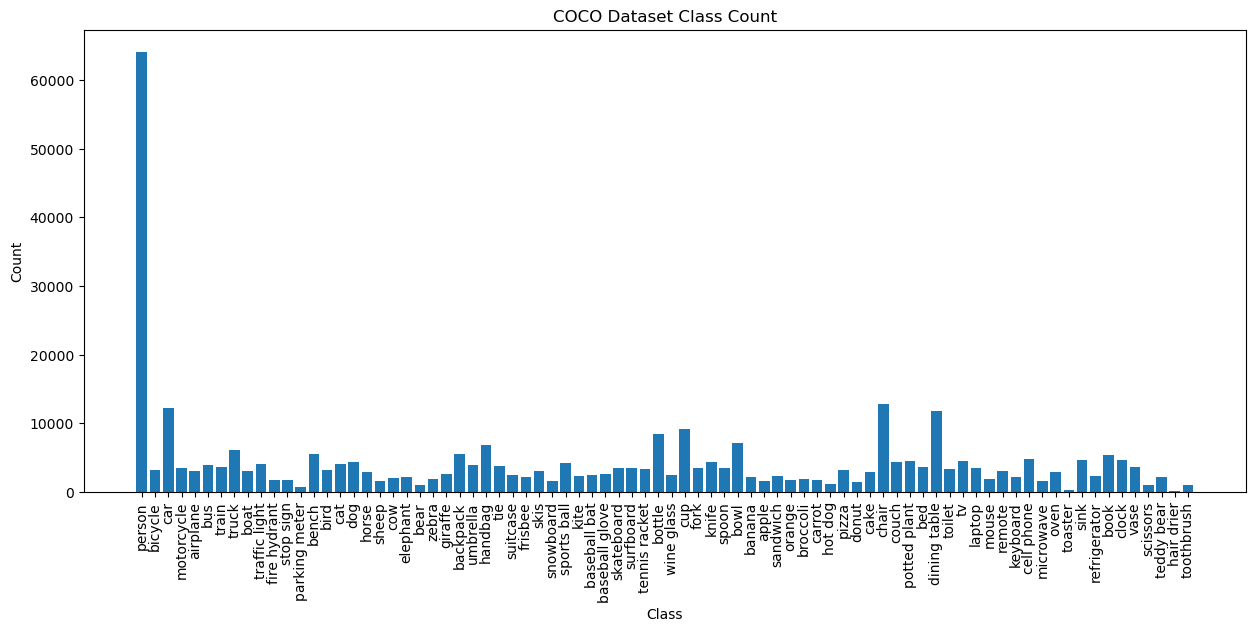
\includegraphics[width=0.5\textwidth,keepaspectratio]{coco_class_count.png}
\caption{COCO Dataset Class Count}
\end{figure}


\subsection{Enhancing the Dataset}\label{Filtering}
As mentioned earlier, COCO dataset contains 80 classes. However, we only need traffic-related object classes.
Therefore, we filtered the dataset to only contain 12 classes. The classes are:
Car Truck Bus Motorcycle Bicycle Traffic Light Stop Sign Train Hydrant Cat Dog
The result is 78,663 images in training split with 12 classes. This amount of data was reduced from 122,125 images in original dataset. By reducing the dataset, our model is expected to take less time to train.
\begin{figure}[h!]
\centering
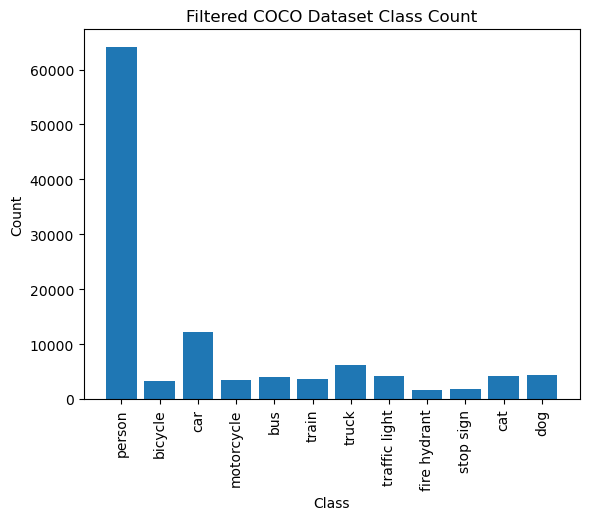
\includegraphics[width=0.5\textwidth]{filtered_coco_class_count.png}
\caption{Filtered COCO Dataset Class Count}
\label{fig:COCOFiltered}
\end{figure}

\begin{figure}[h!]
\centering
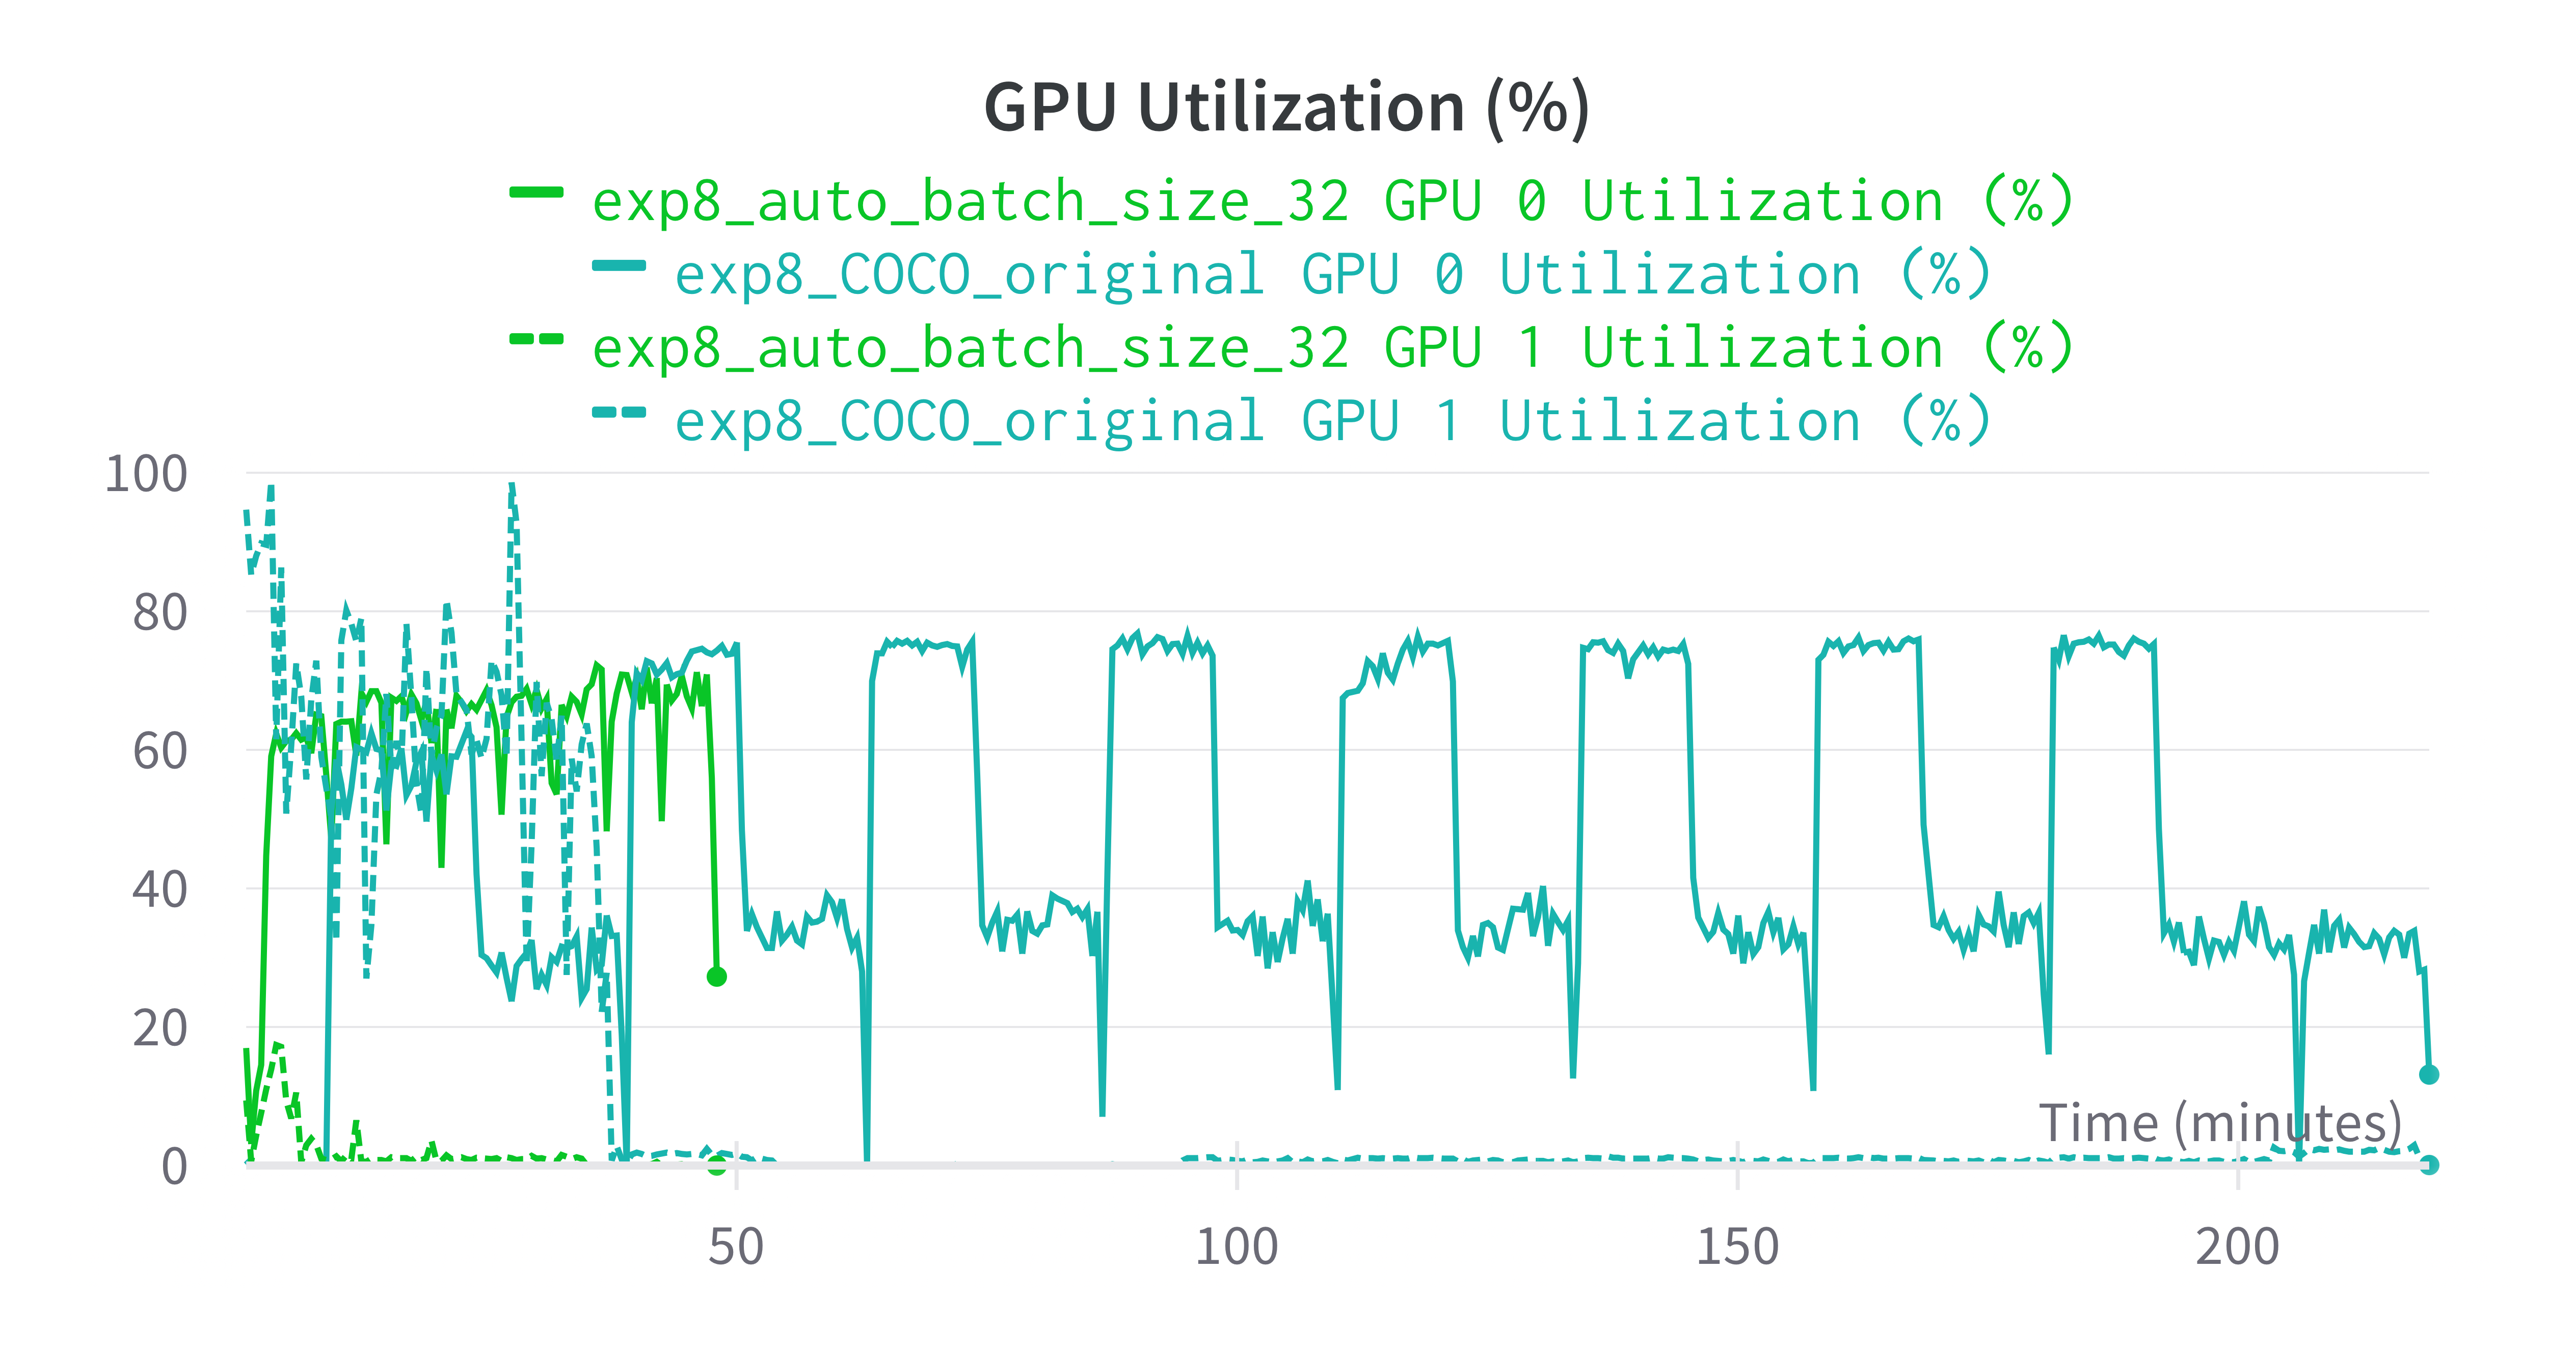
\includegraphics[width=0.3\textwidth,keepaspectratio]{gpu_utilization_comparison_original_and_filtered.png}
\caption{Comparison of GPU Utilization between training the model using filtered dataset and original dataset}
\label{fig:original_filtered_gpu_utilization}
\end{figure}

\begin{figure}[h!]
\centering
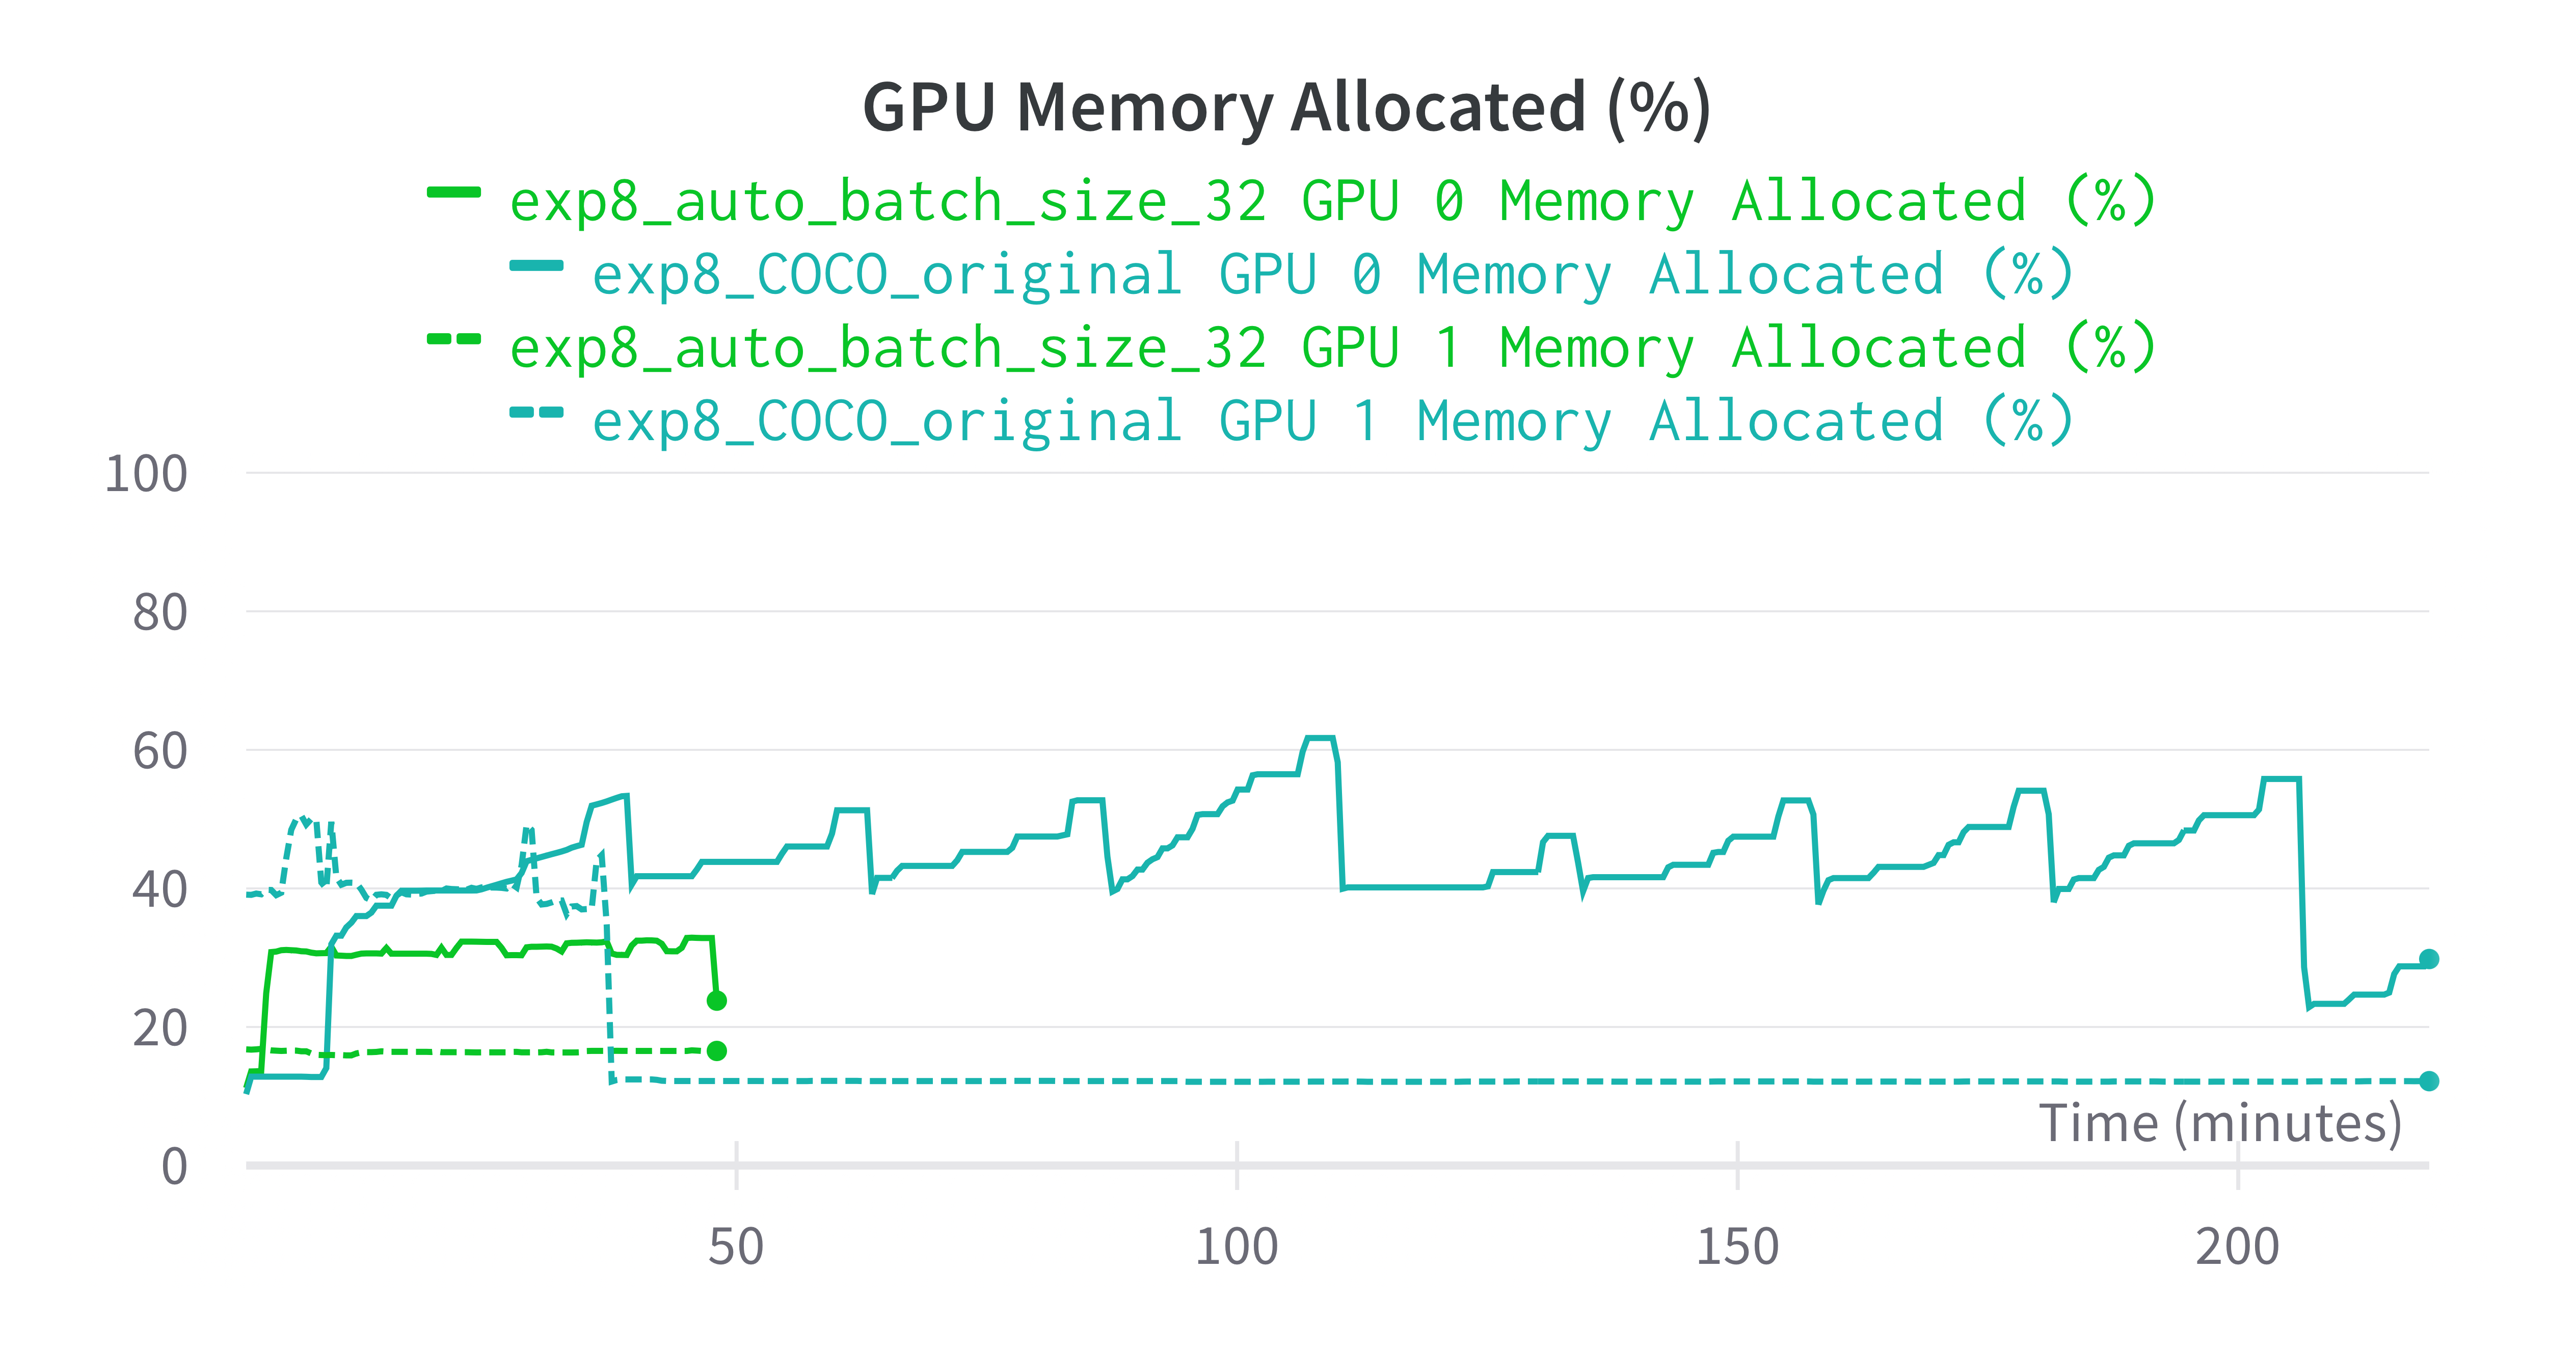
\includegraphics[width=0.3\textwidth,keepaspectratio]{memory_utilization_comparison_original_and_filtered.png}
\caption{Comparison of GPU Memory Utilization between training the model using filtered dataset and original dataset}
\label{fig:original_filtered_memory_utilization}
\end{figure}
In addition, as shown in Fig. \ref{fig:original_filtered_gpu_utilization} and Fig.\ref{fig:original_filtered_memory_utilization}, the filtered dataset has lower GPU Utilization and Memory Utilization. This means that the filtered dataset is more efficient to train.
Thus allowing us to push model training further.
In terms of metrics results, the model trained using a filtered dataset showed better result as indicated by Fig.~\ref{fig:mAP_comparison}. The model trained on a filtered dataset with 8 epochs reaced mAP.95 of 0.298. While the one trained with the original train2017 split only reached 0.135.
\begin{figure}
    \centering
    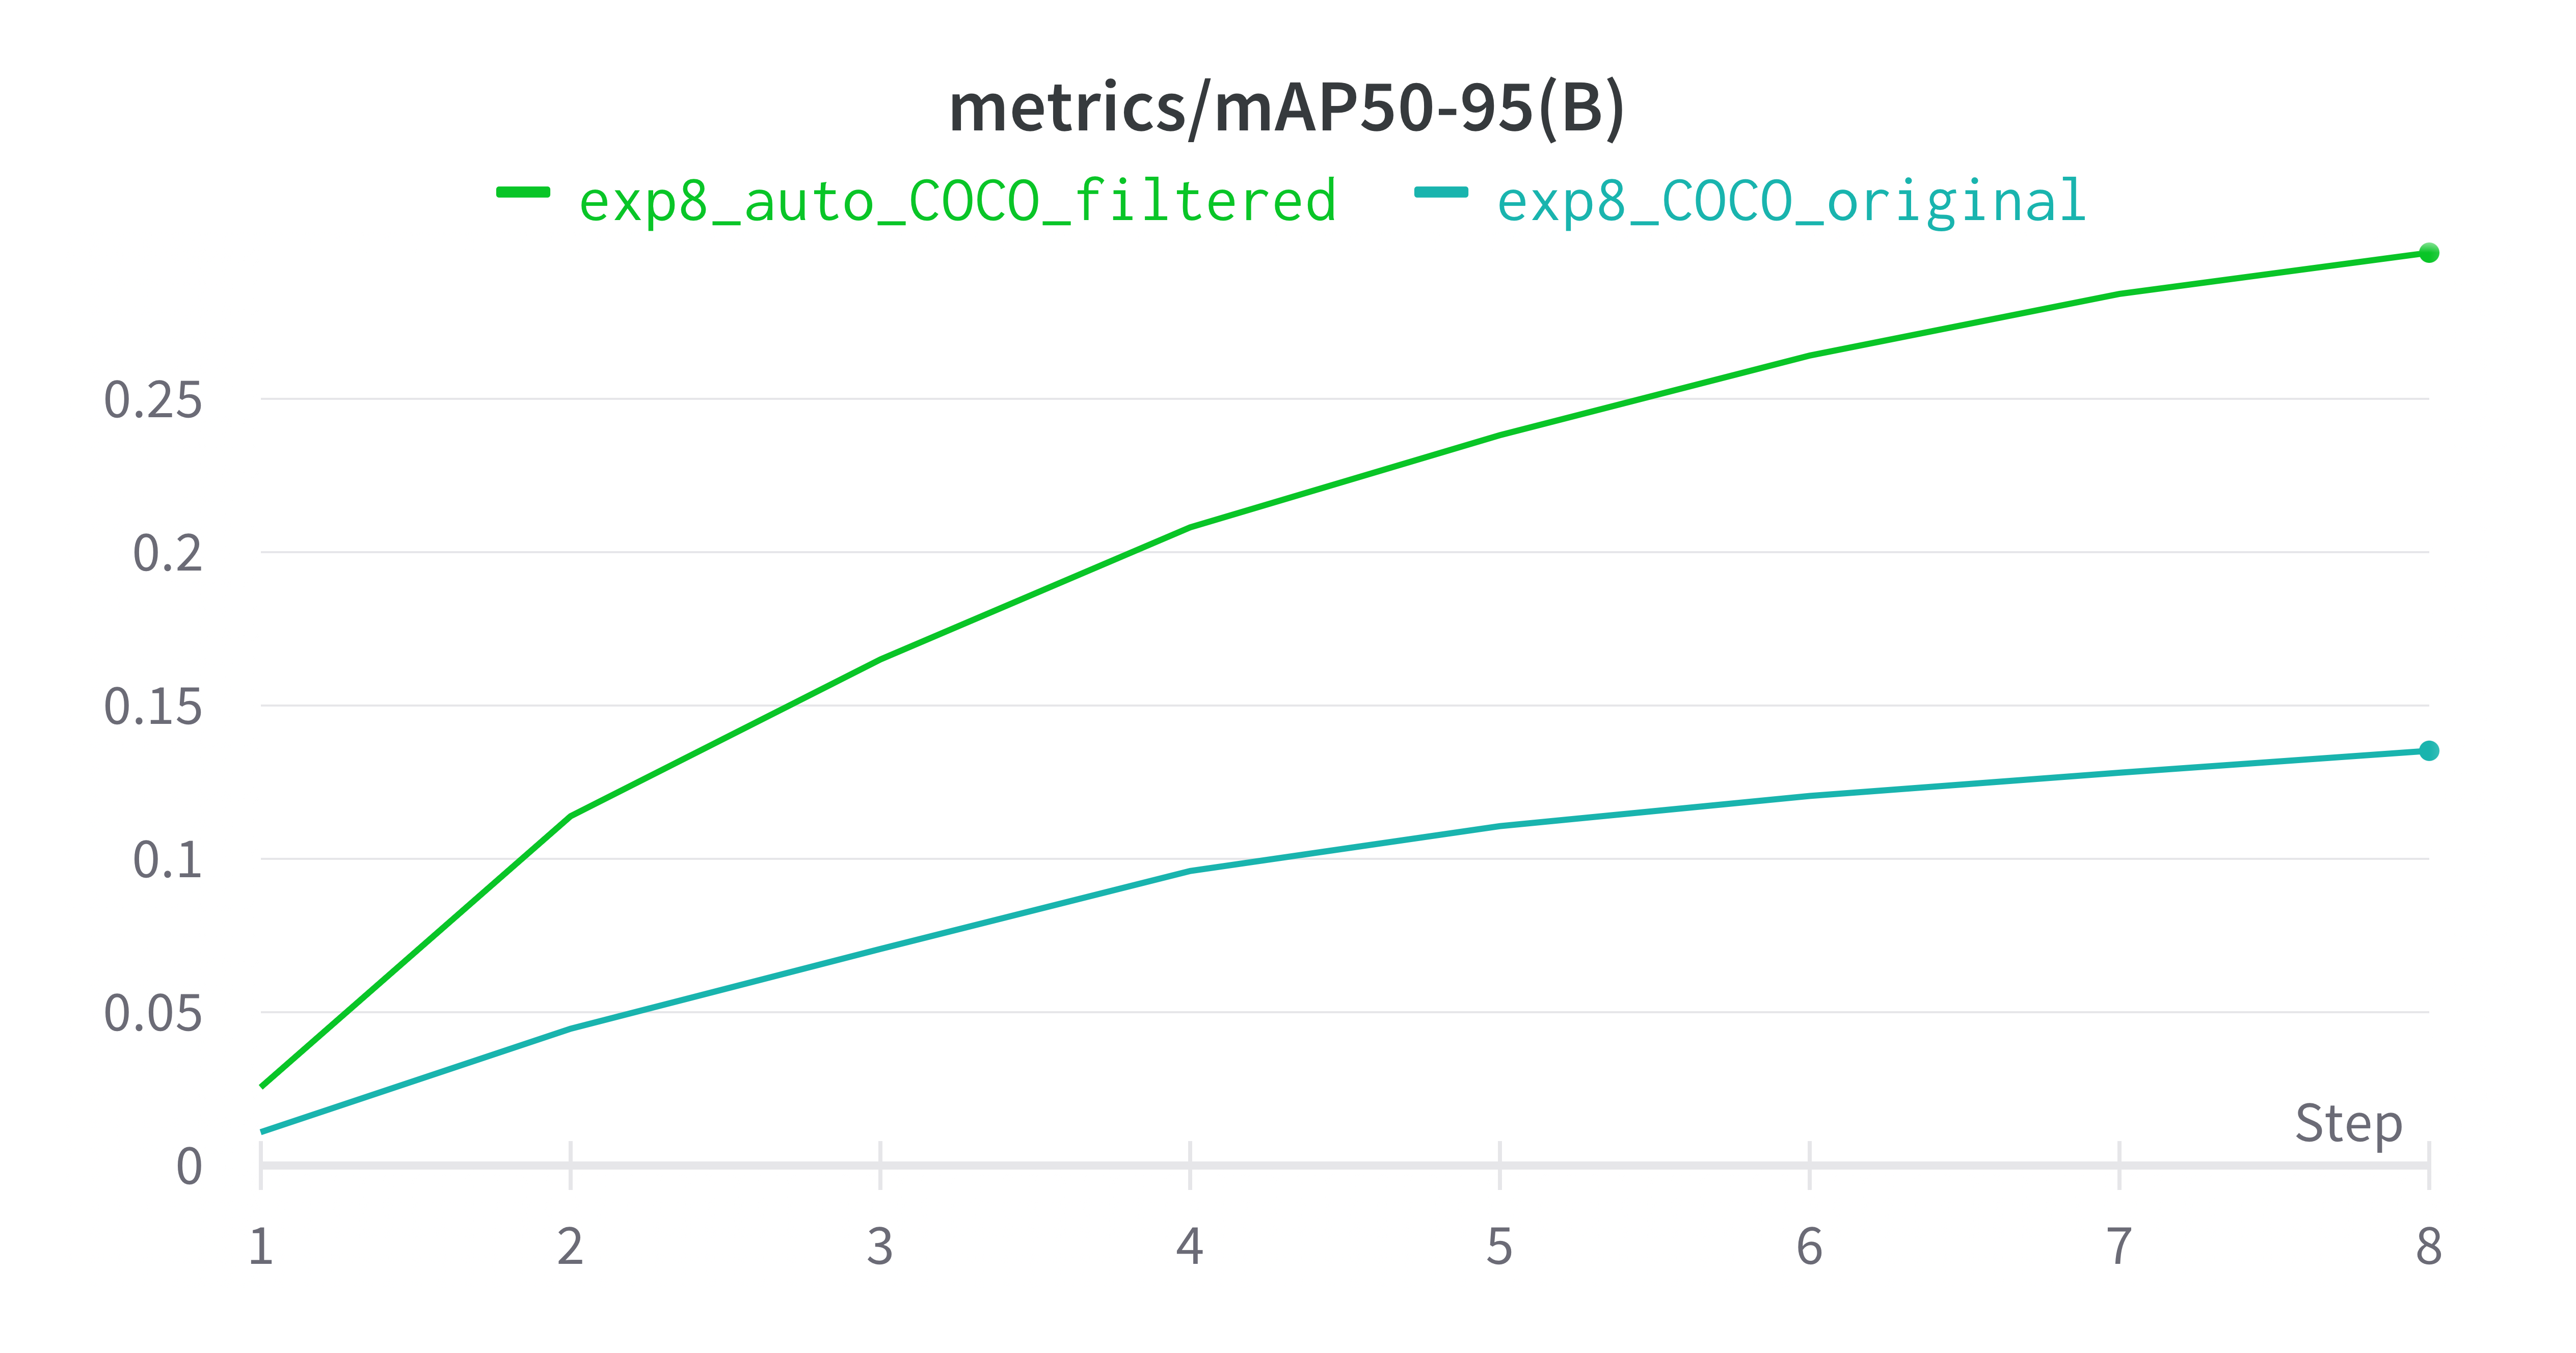
\includegraphics[width=0.5\textwidth,keepaspectratio]{comparison_mAP_filtered.png}
    \caption{Comparison of mAP50-95 between training the model using filtered dataset and original dataset}
\end{figure}

\subsection{Performance Metrics}
For training and validation purposes, we focus on mAP (mean Average Precision), Precision, and recall. mAP is the average of AP (Average Precision) over all classes. AP is the area under the precision-recall curve.
We compare mAP averaged for IoU (Intersection over Union) thresholds from .50 to .95 with .05 increments (MS COCO standard metric, abbreviated as mAP50-95) and mAP50 (PASCAL VOC metric, abbreviated as mAP50) \cite{COCO Dataset}. 
Precision and Recall in  this experiment is a relative measure because it depends on the threshold value.
Precision is calculated by dividing the True Positive by the sum of True Positive and False Positive. 
Precision is calculated using \eqref{equation1}.
\begin{equation}
Precision = \frac{TP}{TP+FP}
\label{equation1}
\end{equation}
Recall calculated by dividing True Positive by the sum of True Positive and False Negative.
\begin{equation}
Recall = \frac{True Positive}{TruePositive+FalseNegative}
\end{equation}
The threshold value determines whether the prediction is Positive or Negative. For example, if the threshold is 0.5, then the prediction is positive if the IoU is greater than 0.5. Otherwise, the prediction is negative.

Both Precision and Recall are relative to the threshold value and are usually used in the form of Precision-Recall Curve. We can calculate the area under the curve to get the Average Precision
To get the value of mAP, we need to calculate Average Precision for each class. Then, we calculate the mean from all Average Precision calculated earlier.
\begin{equation}
mAP = \frac{1}{n}\sum_{i=1}^{n}AP_i
\label{mAP}
\end{equation}
$\eta$ is the number of classes.
This is the main reason of filtering Dataset would be beneficial in our training process. As we use a filtered dataset, the value of $\eta$ in equation \ref{mAP} is 12 instead of 80.
Figure 3 shows the comparison of mAP50 and mAP50-95 between training the model using the filtered dataset and  the original dataset. We can see that the filtered dataset has better mAP50 and mAP50-95 than the original dataset.
\

\section{System Design}
% Flowchart di sini aja
% Fig 1 ceritakan lebih detail
% cerita singkat kita implementasi di jetson nano]
\subsection{Related Work}
Nasution et al.\cite{Road Information Collector} proposed a system that can detect vehicles and street lanes.

Image feed captured using a smartphone, then processed using by ImageAI library with RetinaNet for COCO as an object detection model 
In 2023, Nasution and Dirgantara, proposed pedestrian detections for Autonomous Driving Assistance System (ADAS) using YOLOv5 and Raspberry Pi 4 as the edge computer. The pedestrian detection system is only capable of delivering 0,9 frames per second [6].
\subsection{System Overview}
In this section, we will discuss the system overview. The system consists of 3 main hardware components. 
The first component is the camera. The camera is used to capture the image.
The second component is the edge computer. The edge computer is used to process the image. 
The third component is the display. The display is used to show the result of the image processing.
\begin{figure}[h]
\centering
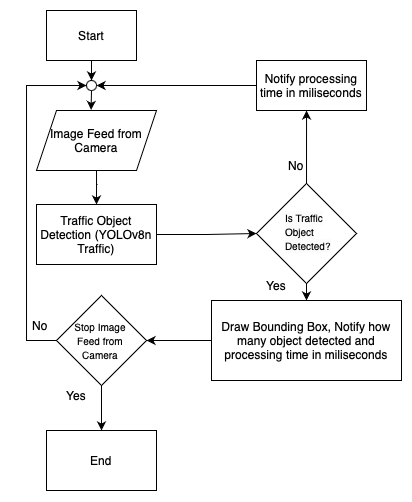
\includegraphics[width=0.4\textwidth,keepaspectratio]{Proposed Flowchart.png}
\caption{Proposed Flowchart of the system}
\label{fig:flowchart}
\end{figure}
\newline
Fig.\ref{fig:flowchart} shows the flowchart of our proposed method of detecting traffic objects. First, the camera captures image frame by frame, followed by preprocessing the images before feeding it to the YOLO model.
The YOLO model gives the bounding box and class of the detected object. The bounding box and class are then drawn on the image. The image with bounding box and class are then displayed on the screen.

\subsection{Edge Processing Unit}
As Nasution and Dirgantara (2023) used Raspberry Pi 4 as their processing unit and only managed to get 0,9 FPS, we decided to find a more powerful edge computer that was similar in terms of price. At the time of writing this paper, Raspberry Pi 4 4GB cost around 200 USD. While Jetson Nano 4GB cost around 250 to 300 USD.
Another factor that we consider is the availability of GPU. As we know, GPU is the main component in deep learning. Therefore, we need to find an edge computer that has a GPU.
Jetson Nano is powered by Quad Core ARM-A57 CPU with 32 cores of Maxwell GPU. This Maxwell GPU is the main selling point of Jetson Nano because it has CUDA Core, hence allowing us to run accelerated deep learning model.

\subsection{Experimental Setup}
In this section, we will discuss  the experimental setup. We are using Pytorch as our deep learning framework in Python  3.
Model training was conducted on Geforce RTX 3090, 24 GB Video RAM, 32GB RAM, Intel Core i3-12100 4 Core 8 Thread, running on Windows 10
Model inference and testing was performed on Macbook Air M1 and Jetson Nano 4GB. The camera used in this experiment is Lifecam Studio by Microsoft.
Jetson Nano that we use running on Ubuntu 20.04.2 LTS on top of Jetpack 4.6. We use Jetson Nano 4GB as our edge computer because it is the most affordable edge computer in the Nvidia Jetson Series.
\subsection{Testing Dataset}
As mentioned earlier, we are using the COCO dataset to train and validate our model, especially train20117 and val2017. However, we filtered the dataset to only contain 12 classes. The classes are
Car, Truck, Bus, Motorcycle, Bicycle, Traffic Light, Stop Sign, Train, Hydrant, Cat, Dog. The result is 78000 images with 12 classes.
For inference and real-world testing, we gather our own data by recording traffic conditions in Bandung, Indonesia. The data was recorded using the camera mentioned earlier.
As some part of the traffic footage that we collected, we also utilized it as an addition to our training dataset. This is because Indonesia's traffic condition is different from other countries. In Indonesia, a motorcycle is more often used than a car.
If we refer to the filtered COCO dataset in Fig.\ref{fig:COCOFiltered}, the number of motorcycle is lower than the number of car class. Therefore, we need to add more motorcycle data to our dataset.
\begin{figure}[h]
\centering
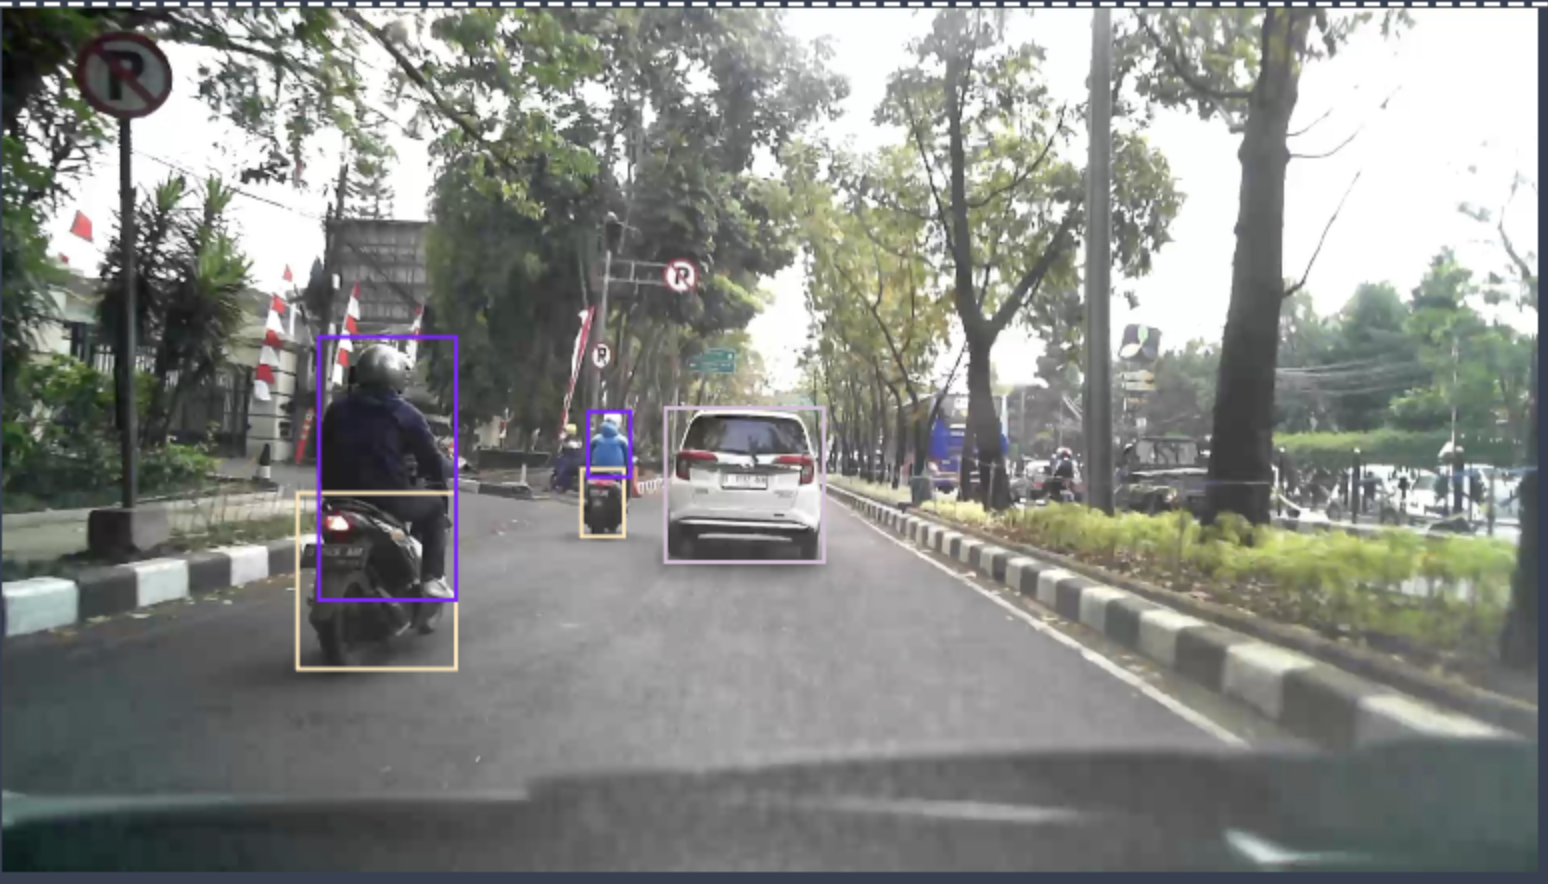
\includegraphics[width=0.4\textwidth,keepaspectratio]{sample_dataset.png}
\caption{Sample of our annotated image from footage that we collected}
\end{figure}

\subsection{Training}
Before we begin the training process of our YOLOv8n-Traffic model with high a number of epochs, we want to find the optimal hyperparameter configuration for our use case. We conducted various training configuratios with 8 epochs to save time.
Although each run for one configuration is only 8 epoch, it still takes about 1 to 2 hours. However, we can get the result faster than training with 100 epochs for each configuration.

We tried different batch size, learning rate, and optimizers. We use batch size 16 and 32.
\begin{figure}[h]
\centering
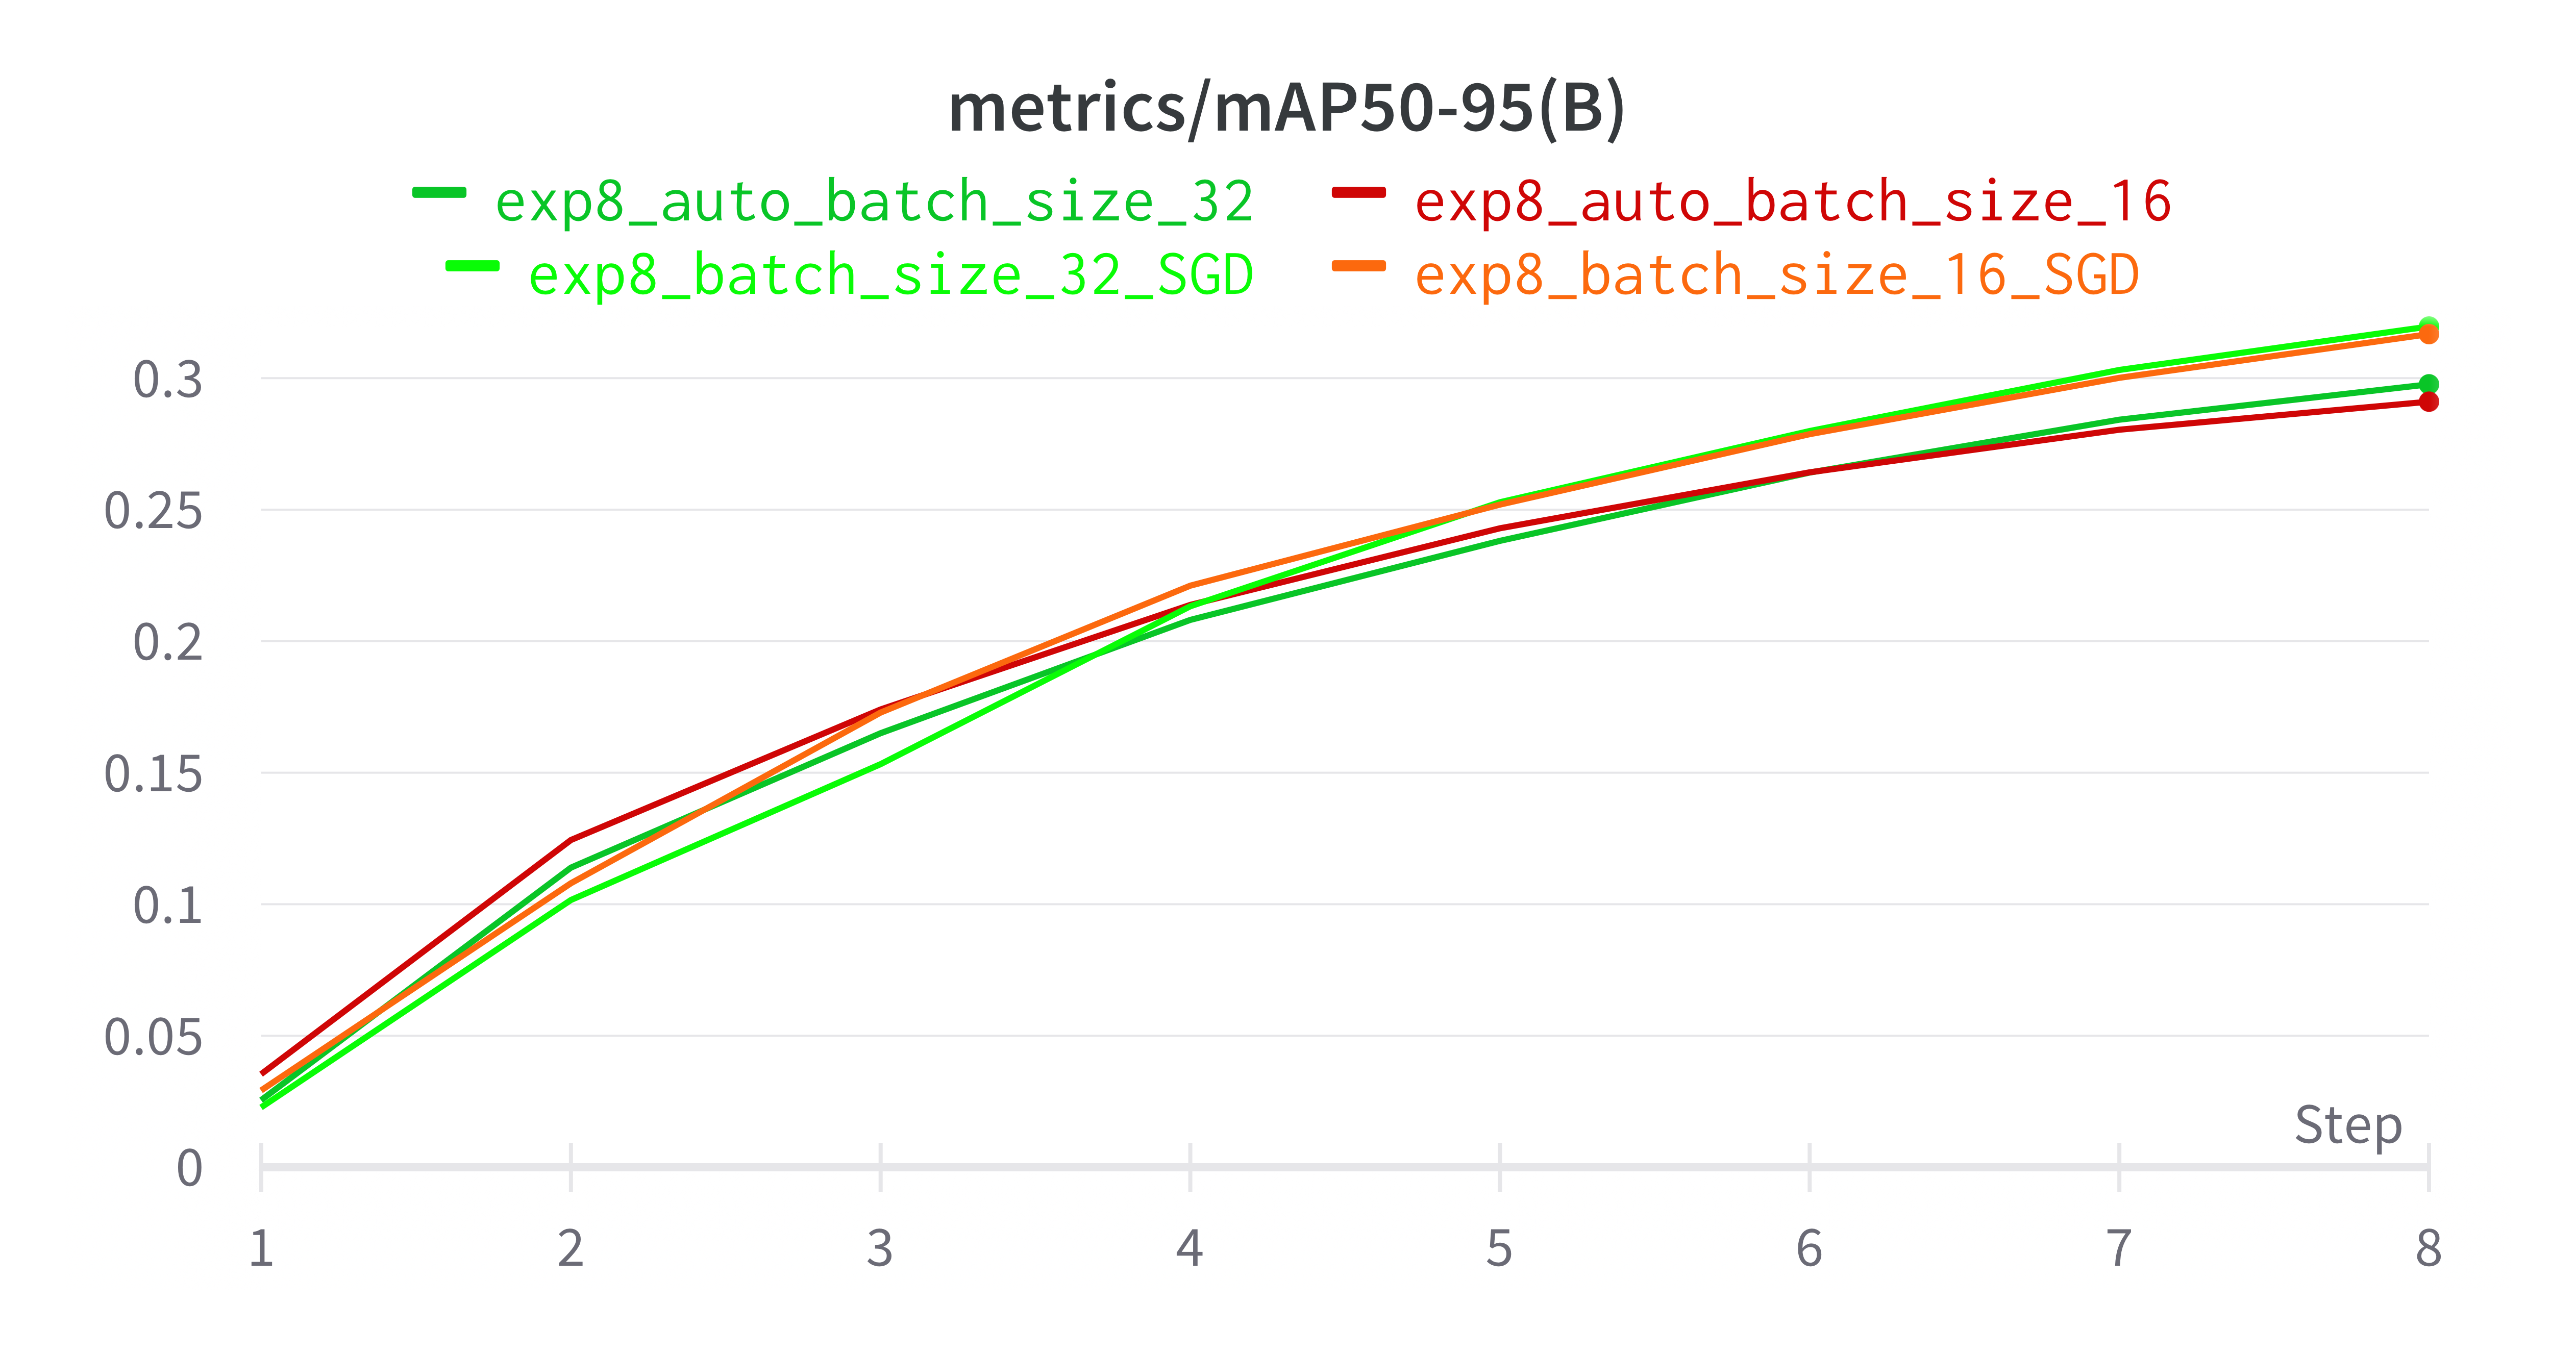
\includegraphics[width=0.4\textwidth,keepaspectratio]{mAP_batch_size_comparison.png} % TODO ; change file name
\caption{Comparison of mAP50-95 between training the model using batch size 16 and 32}
\label{fig:batch_size}
\end{figure}

\begin{figure}[h!]
\centering
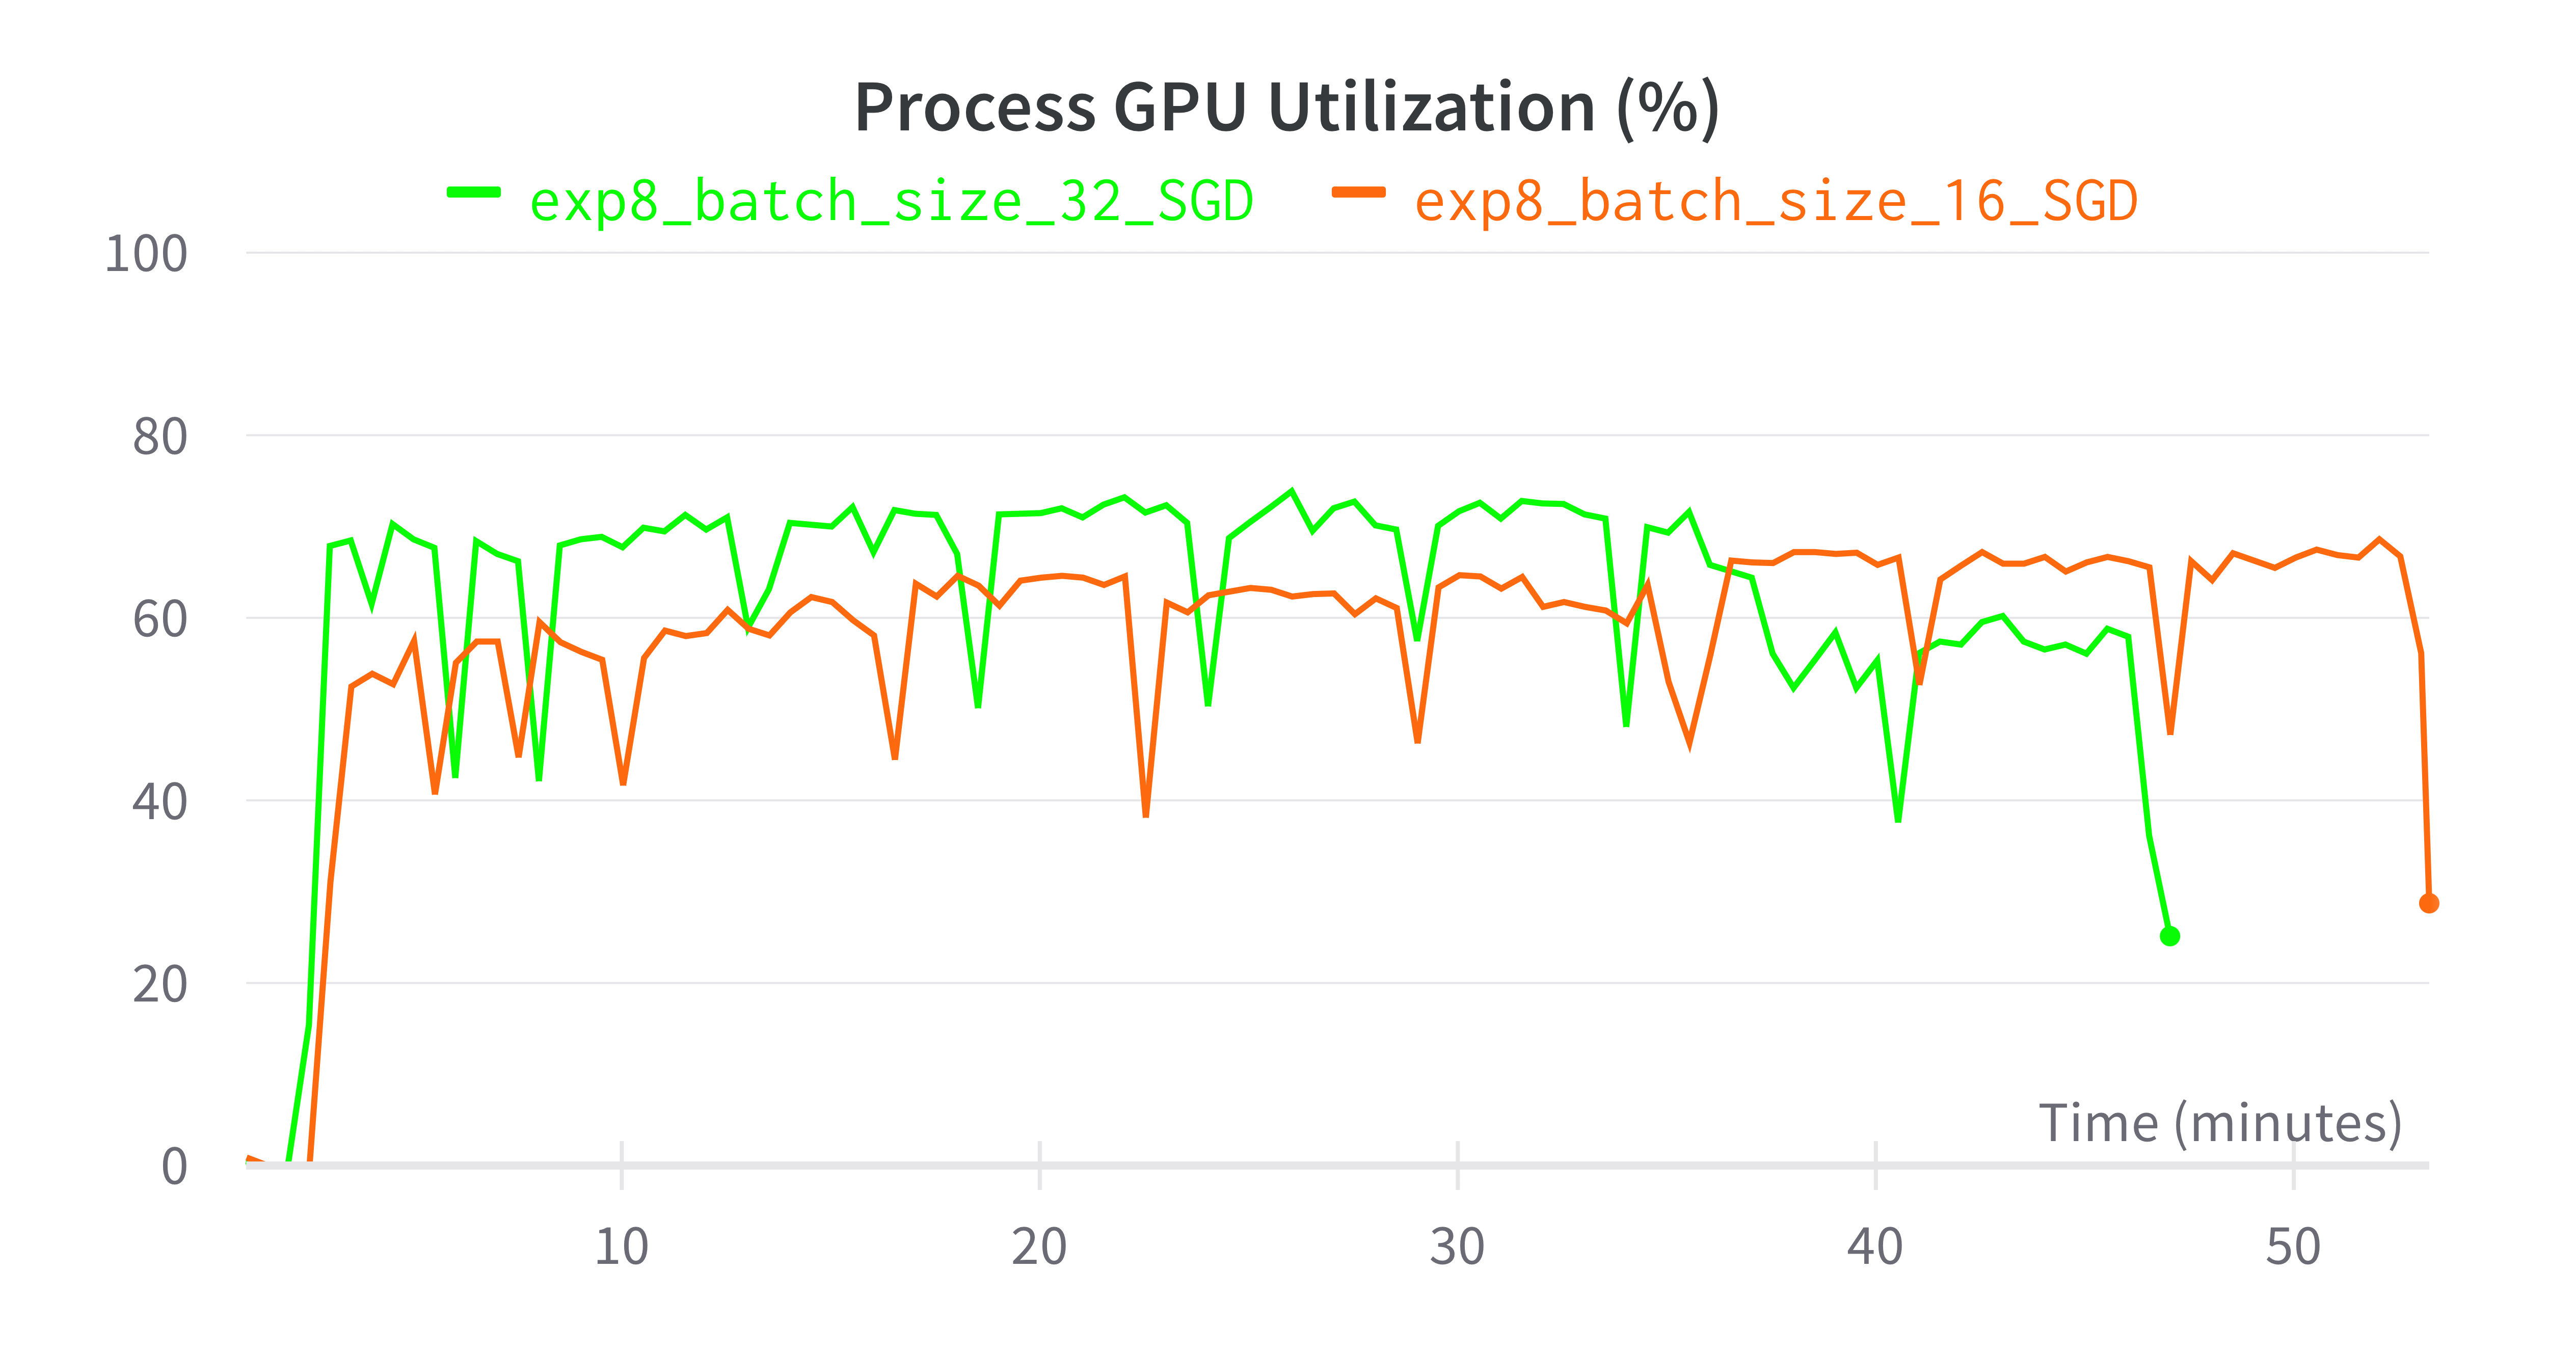
\includegraphics[width=0.4\textwidth,keepaspectratio]{gpu_utilization_comparison.png} 
\caption{Comparison of GPU Utilization between training the model using batch size 16 and 32}
\label{fig:gpu_utilization}
\end{figure}
% gpu_utilization_comparison.png
Fig.\ref{fig:batch_size} shows the result of training with different batch size. We can see that batch size 32 is better than batch size 16. Especially in terms of training time, batch size 32 is faster than batch size 16.
Therefore, we use batch size 32 for our training. We also tried using SGD and Adam optimizer. YOLOv8 implements optimizer switching depending on the number of iterations.


\subsection{Real World Testing}
In this section, we will discuss real-world testing. We bring our system to real-world environment scenario, placed our whole system into the dashboard of vehicles.
\begin{figure}[h!]
    \centering
    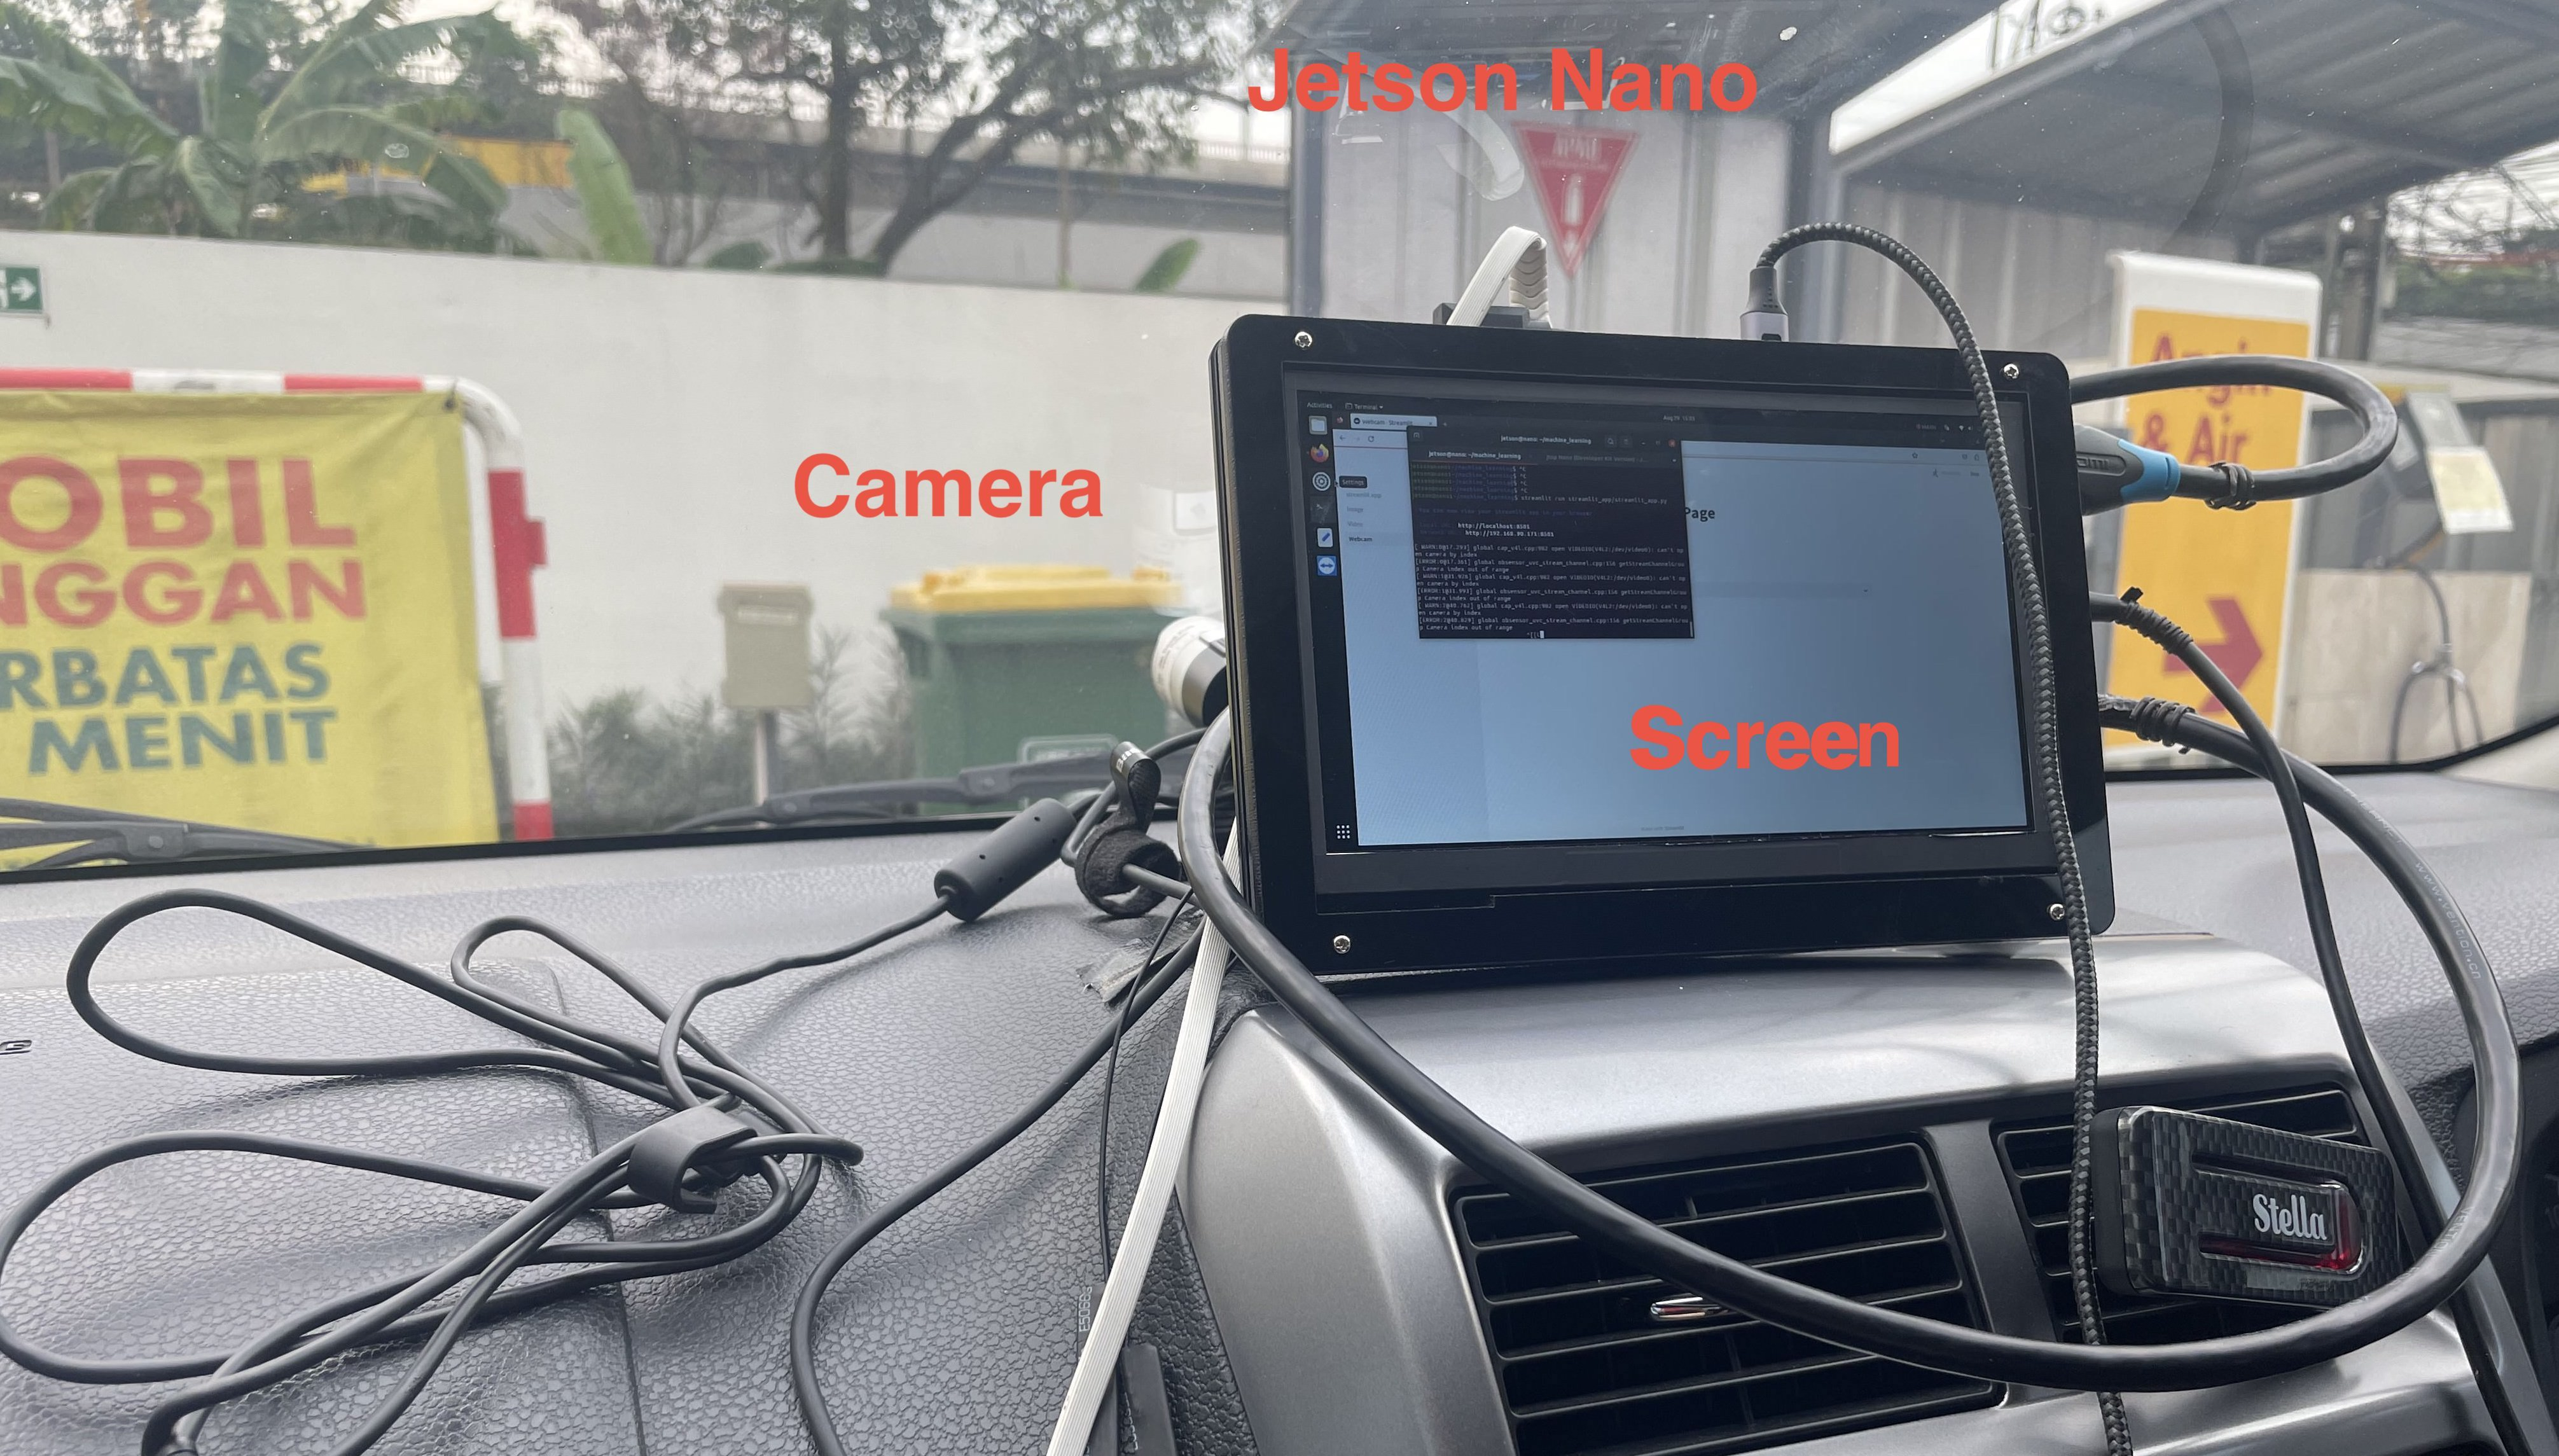
\includegraphics[width=0.4\textwidth,keepaspectratio]{mounted_camera_front_view.jpg}
    \caption{Front View}
    \label{fig:front_view}
\end{figure}

\begin{figure}[h!]
    \centering
    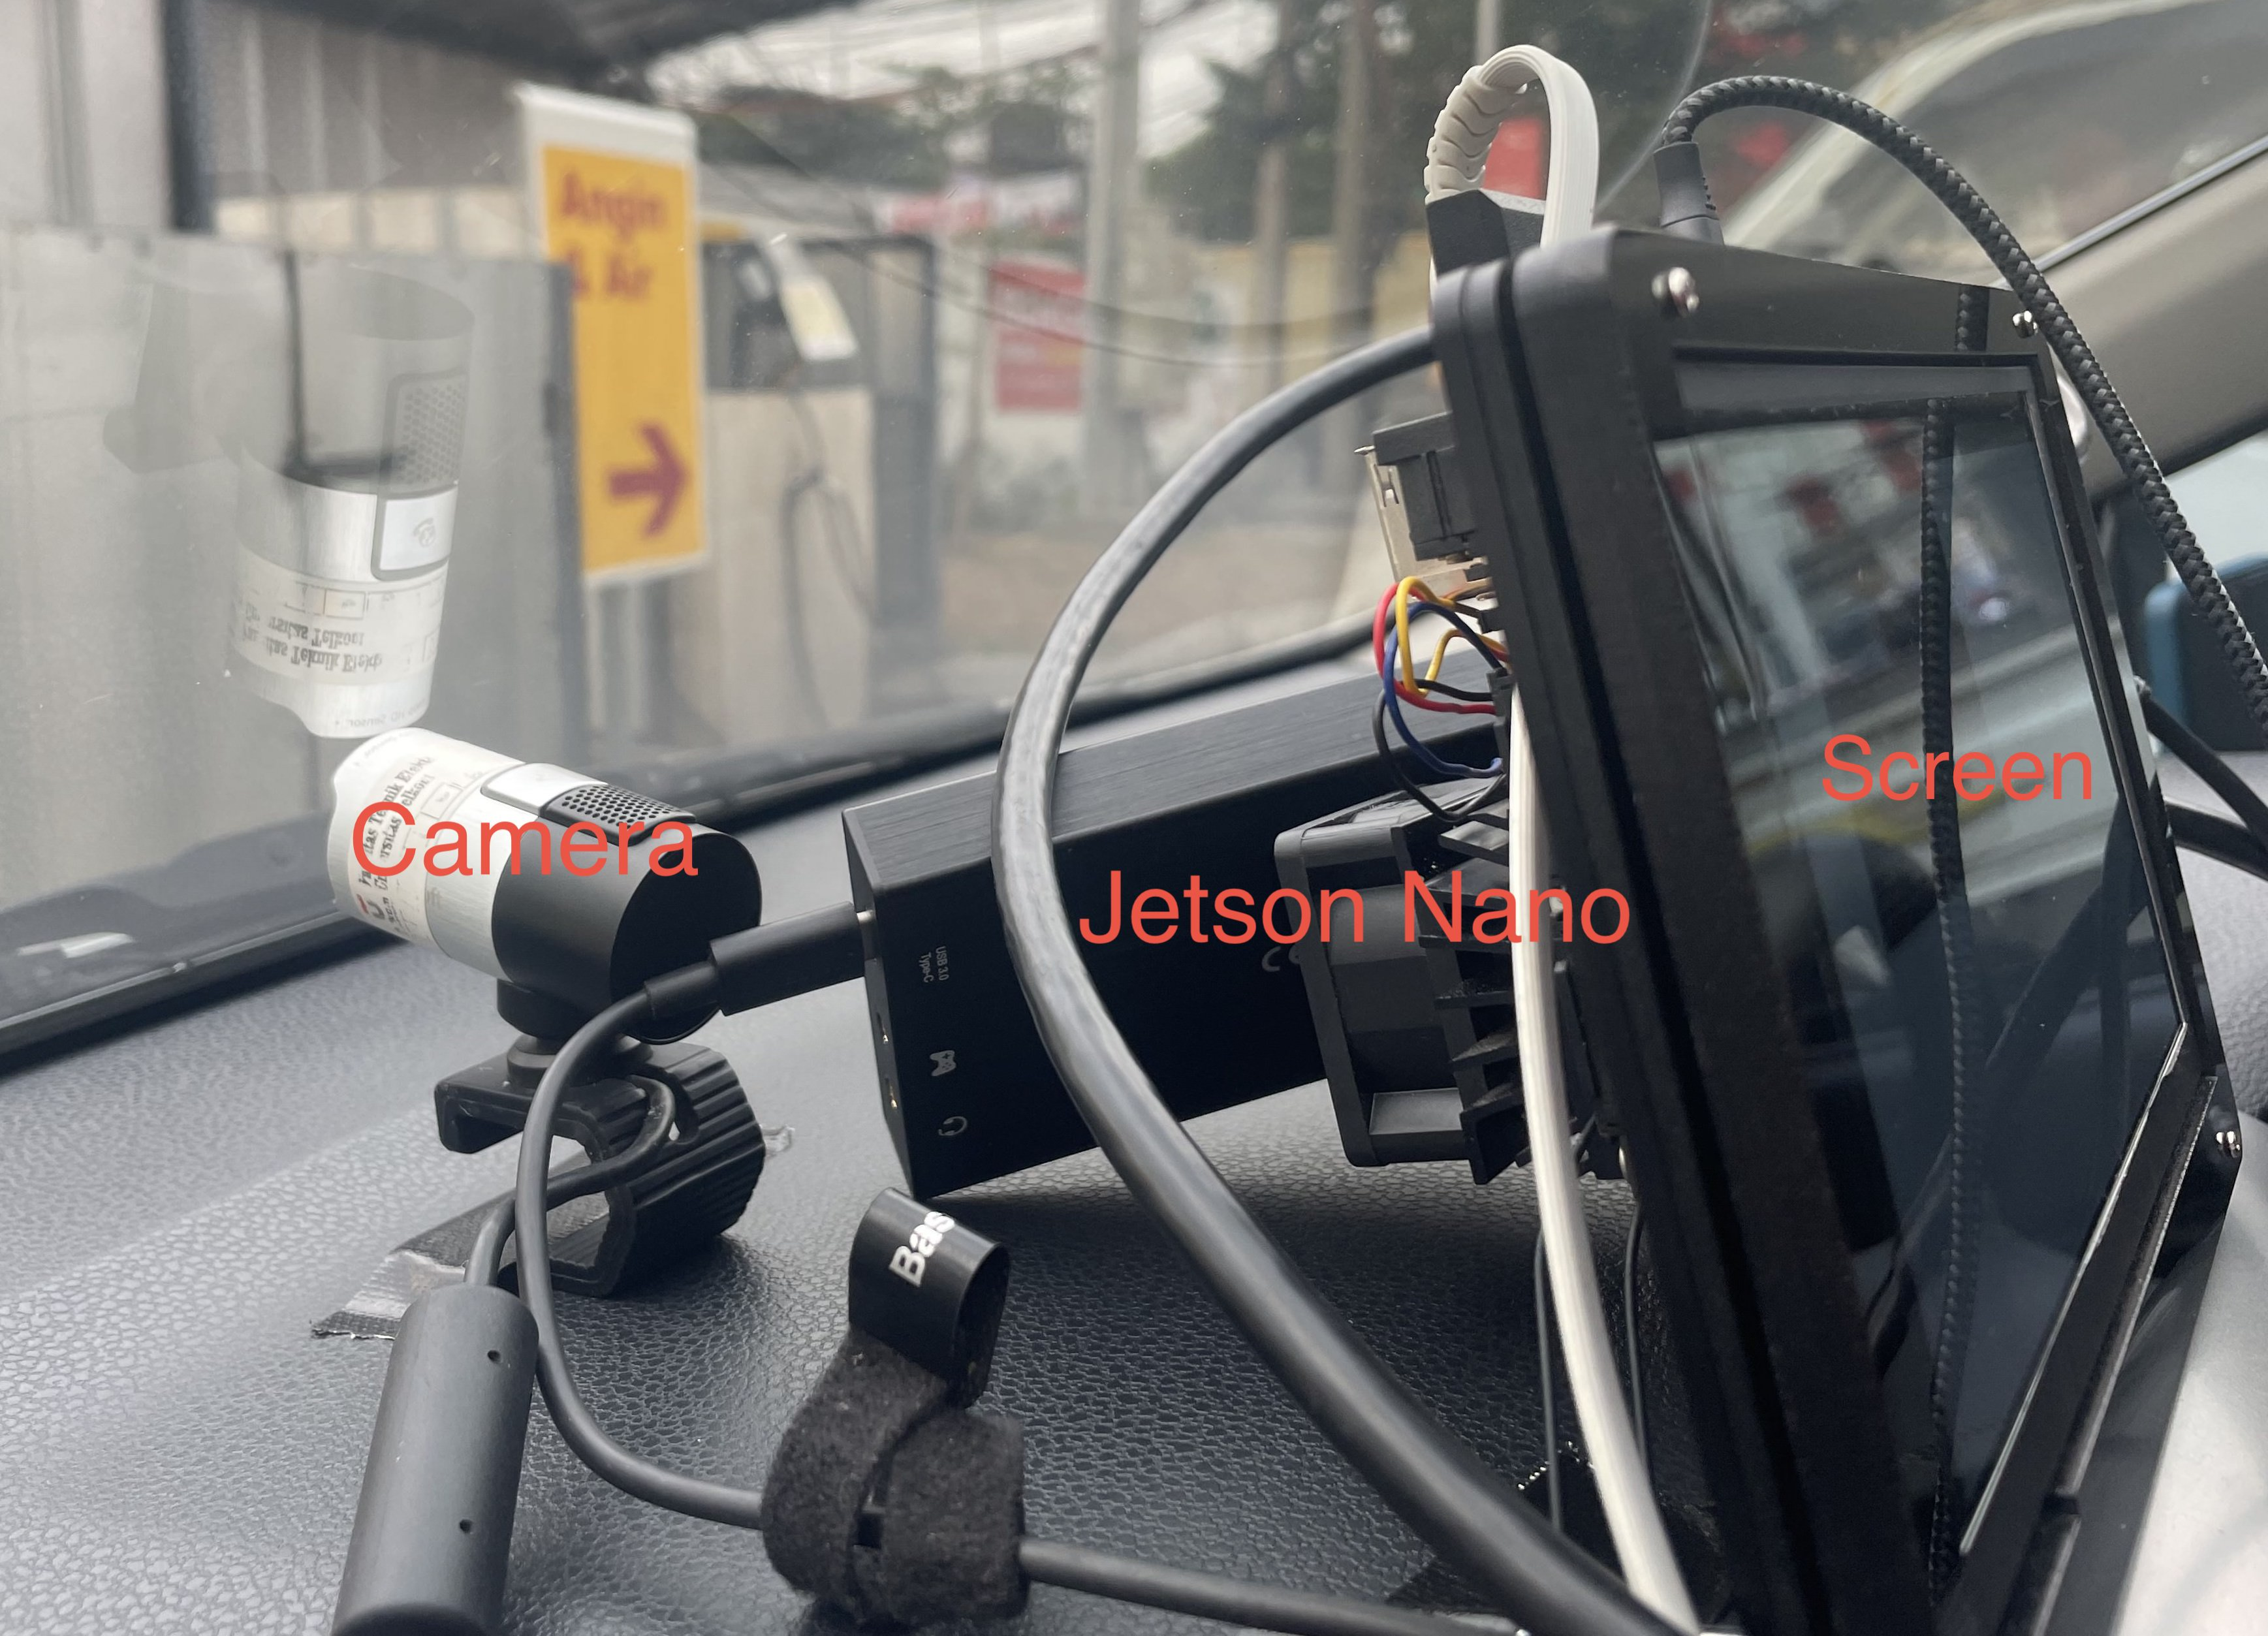
\includegraphics[width=0.4\textwidth,keepaspectratio]{mounted_camera_side_view.jpg}
    \caption{Side View}
    \label{fig:side_view}
\end{figure}
We use USB car charger to power our system. We drove around the city of Bandung to test our system. 

\section{Results and Discussion}
In this section, we will discuss  the result of our experiment. We will discuss  the result of training and real-world testing.
\subsection{Training Result}
In this section, we will discuss the result of our object detection model training. We use the configuration concluded from the previous section. First, train our model with 80 epochs.
Then in order to compare the performance of YOLOv8n model, we also train YOLOv7-tiny model.
YOLOv7-tiny is the smallest modelin theYOLOv7 series. However, it needs more computation power than YOLOv8n. We train both YOLOv7-tiny and YOLOv8n with 80 epochs.
Fig.\ref{fig:mAP_comparison} indicates that YOLOv7-tiny is slightly better than YOLOv8n in terms of mAP50-95. However, YOLOv8n is better than YOLOv7-tiny.
\begin{figure}
\centering
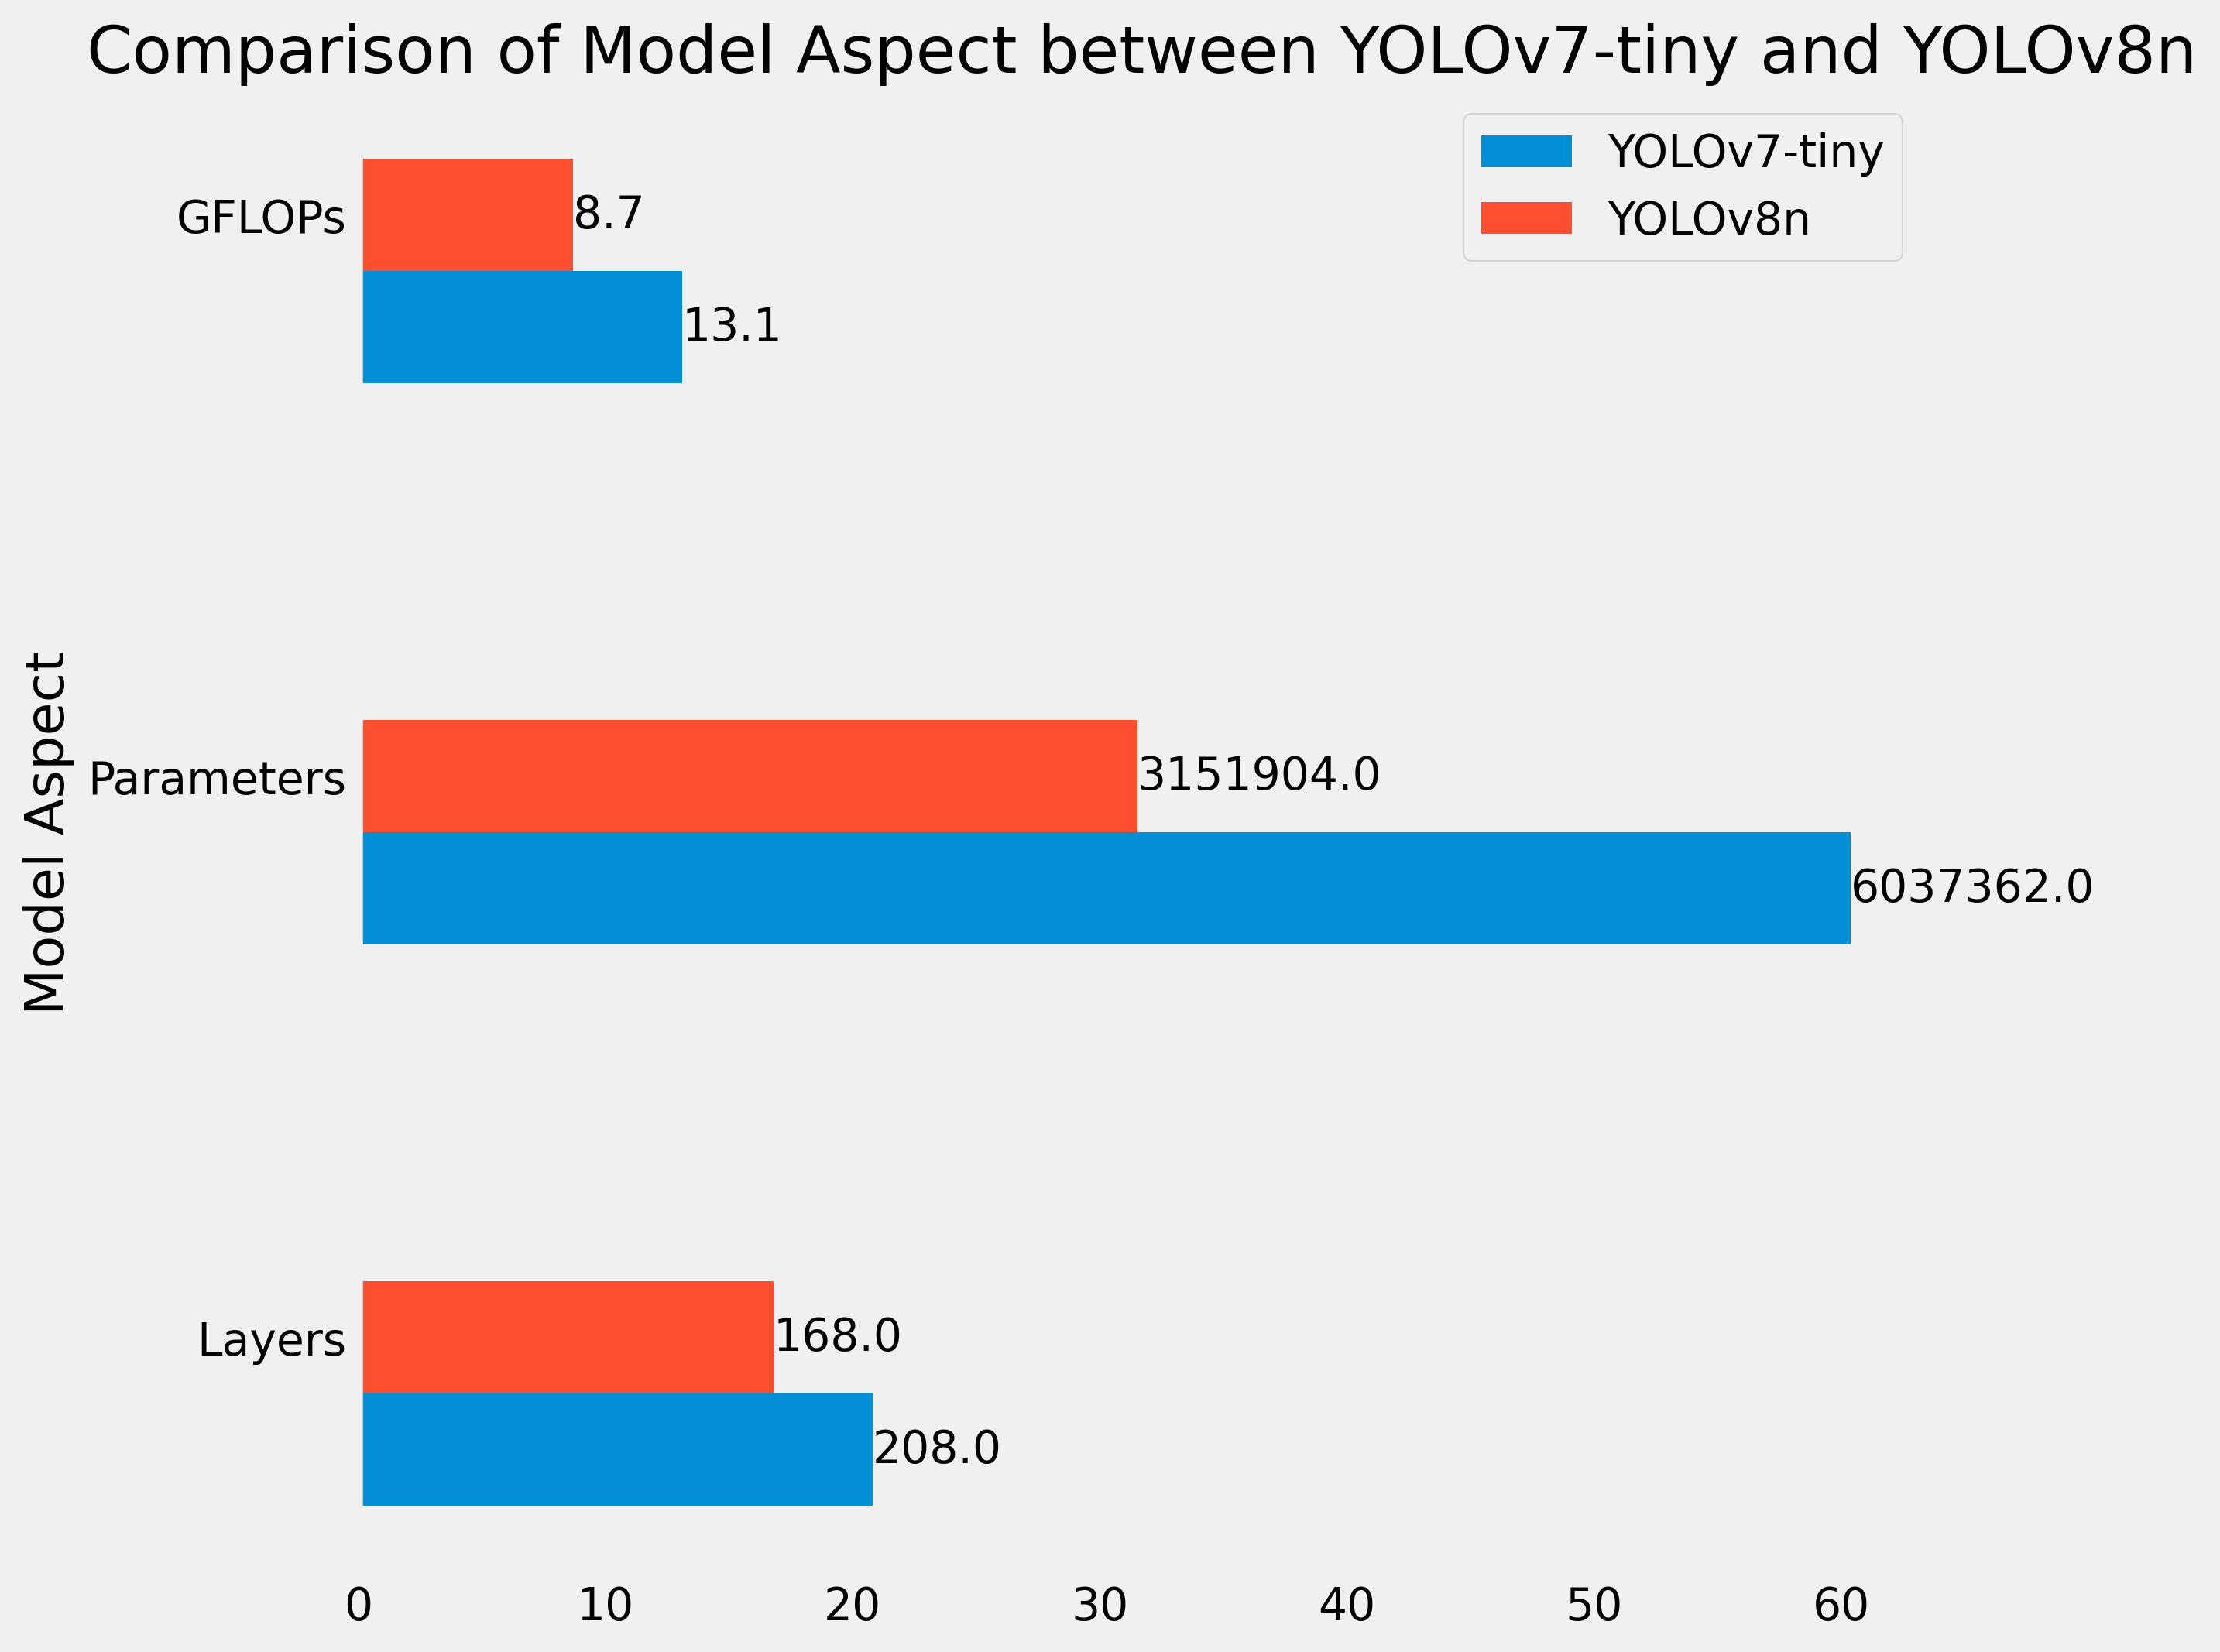
\includegraphics[width=0.4\textwidth,keepaspectratio]{YOLOv7-tinyvsYOLOv8n_model_aspect.png}    
\caption{Layers, Parameters, and GFLOPs Comparison between YOLOv7-tiny and YOLOv8n}
\end{figure}

\begin{figure}[h]
\centering
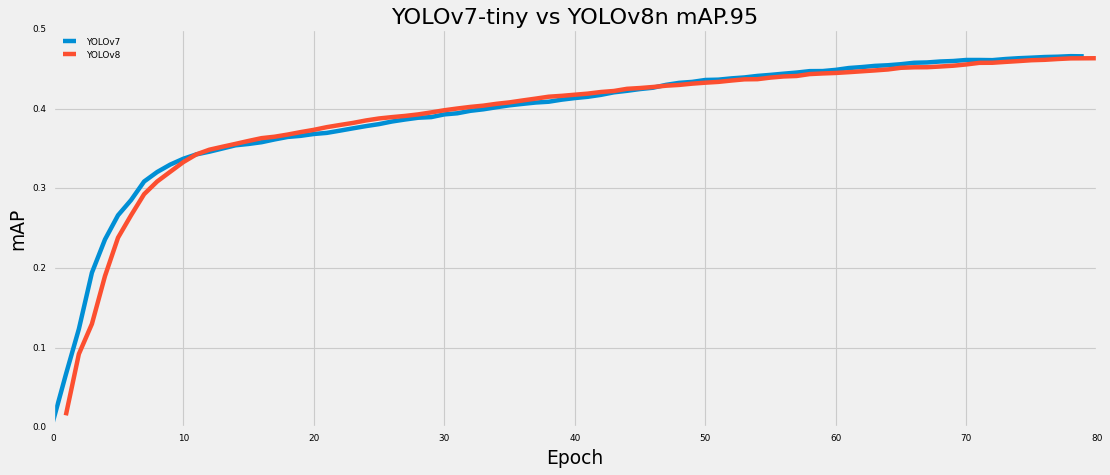
\includegraphics[width=0.4\textwidth,keepaspectratio]{YOLOv7-tinyvsYOLOv8n.png}
\caption{Comparison of mAP50-95 between YOLOv8n and YOLOv7-tiny}
\label{fig:mAP_comparison}
\end{figure}


As our goal is to run the model on an edge computer, we need to consider the inference time. As mentioned earlier, the computational cost of YOLOv8n is 8 GFLOPs while YOLOv7-tiny is 13 GFLOPs.
That's why we prefer using YOLOv8n. Hence, in order to achieve the performance of YOLOv7-tiny, we try to YOLOv8n with higher number of epochs.
This time we add 20 epochs to our training. We train YOLOv8n with 100 epochs. Fig.\ref{fig:YOLOv7vsYOLOv8,80,100} shows the comparison of result between YOLOv7-tiny, YOLOv8n with 80 epochs, and YOLOv8n with 100 epochs.
\begin{figure}[h!]
\centering
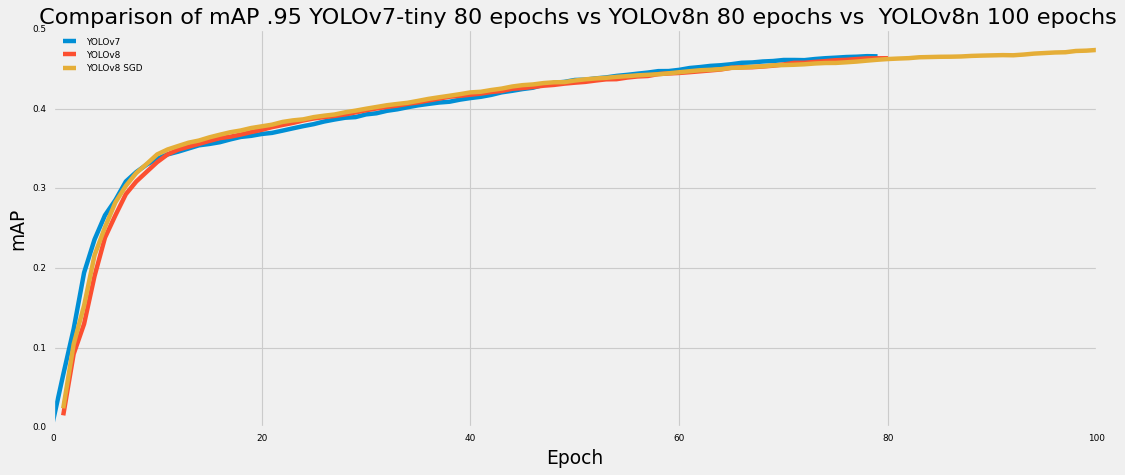
\includegraphics[width=0.4\textwidth,keepaspectratio]{YOLOv7vs YOLOv8,80,100.png}
\caption{Comparison of mAP50-95 between YOLOv7-tiny, YOLOv8n with 80 epochs, and YOLOv8n with 100 epochs}
\label{fig:YOLOv7vsYOLOv8,80,100}
\end{figure}
Finally, with 100 epochs training, our YOLOv8n model achieves similar metrics results with YOLOv7-tiny, despite being lower in computation cost.

\subsection{Real-World Testing Result}
Our test result shows that our system can detect traffic object in real-world  environment.
As mentioned earlier, we use a car charger to power the system. While the system is running, we also use the other port on the same car charger to charge our smartphone. This results in different power available for our system.
By doing this we can simulate the real user scenario. In a user scenario, the user might use the other port on the car charger to charge their smartphone. many cars only have one port for a car charger and no other USB power inside the car.
As a result, our system can run in 3 different power consumption. 5 Watt, 7 Watt, and 10 Watt.

\begin{equation}\label{FPS}
    Frame Per Second = \frac{1000}{latency}
\end{equation}

\begin{figure}[h!]
\centering
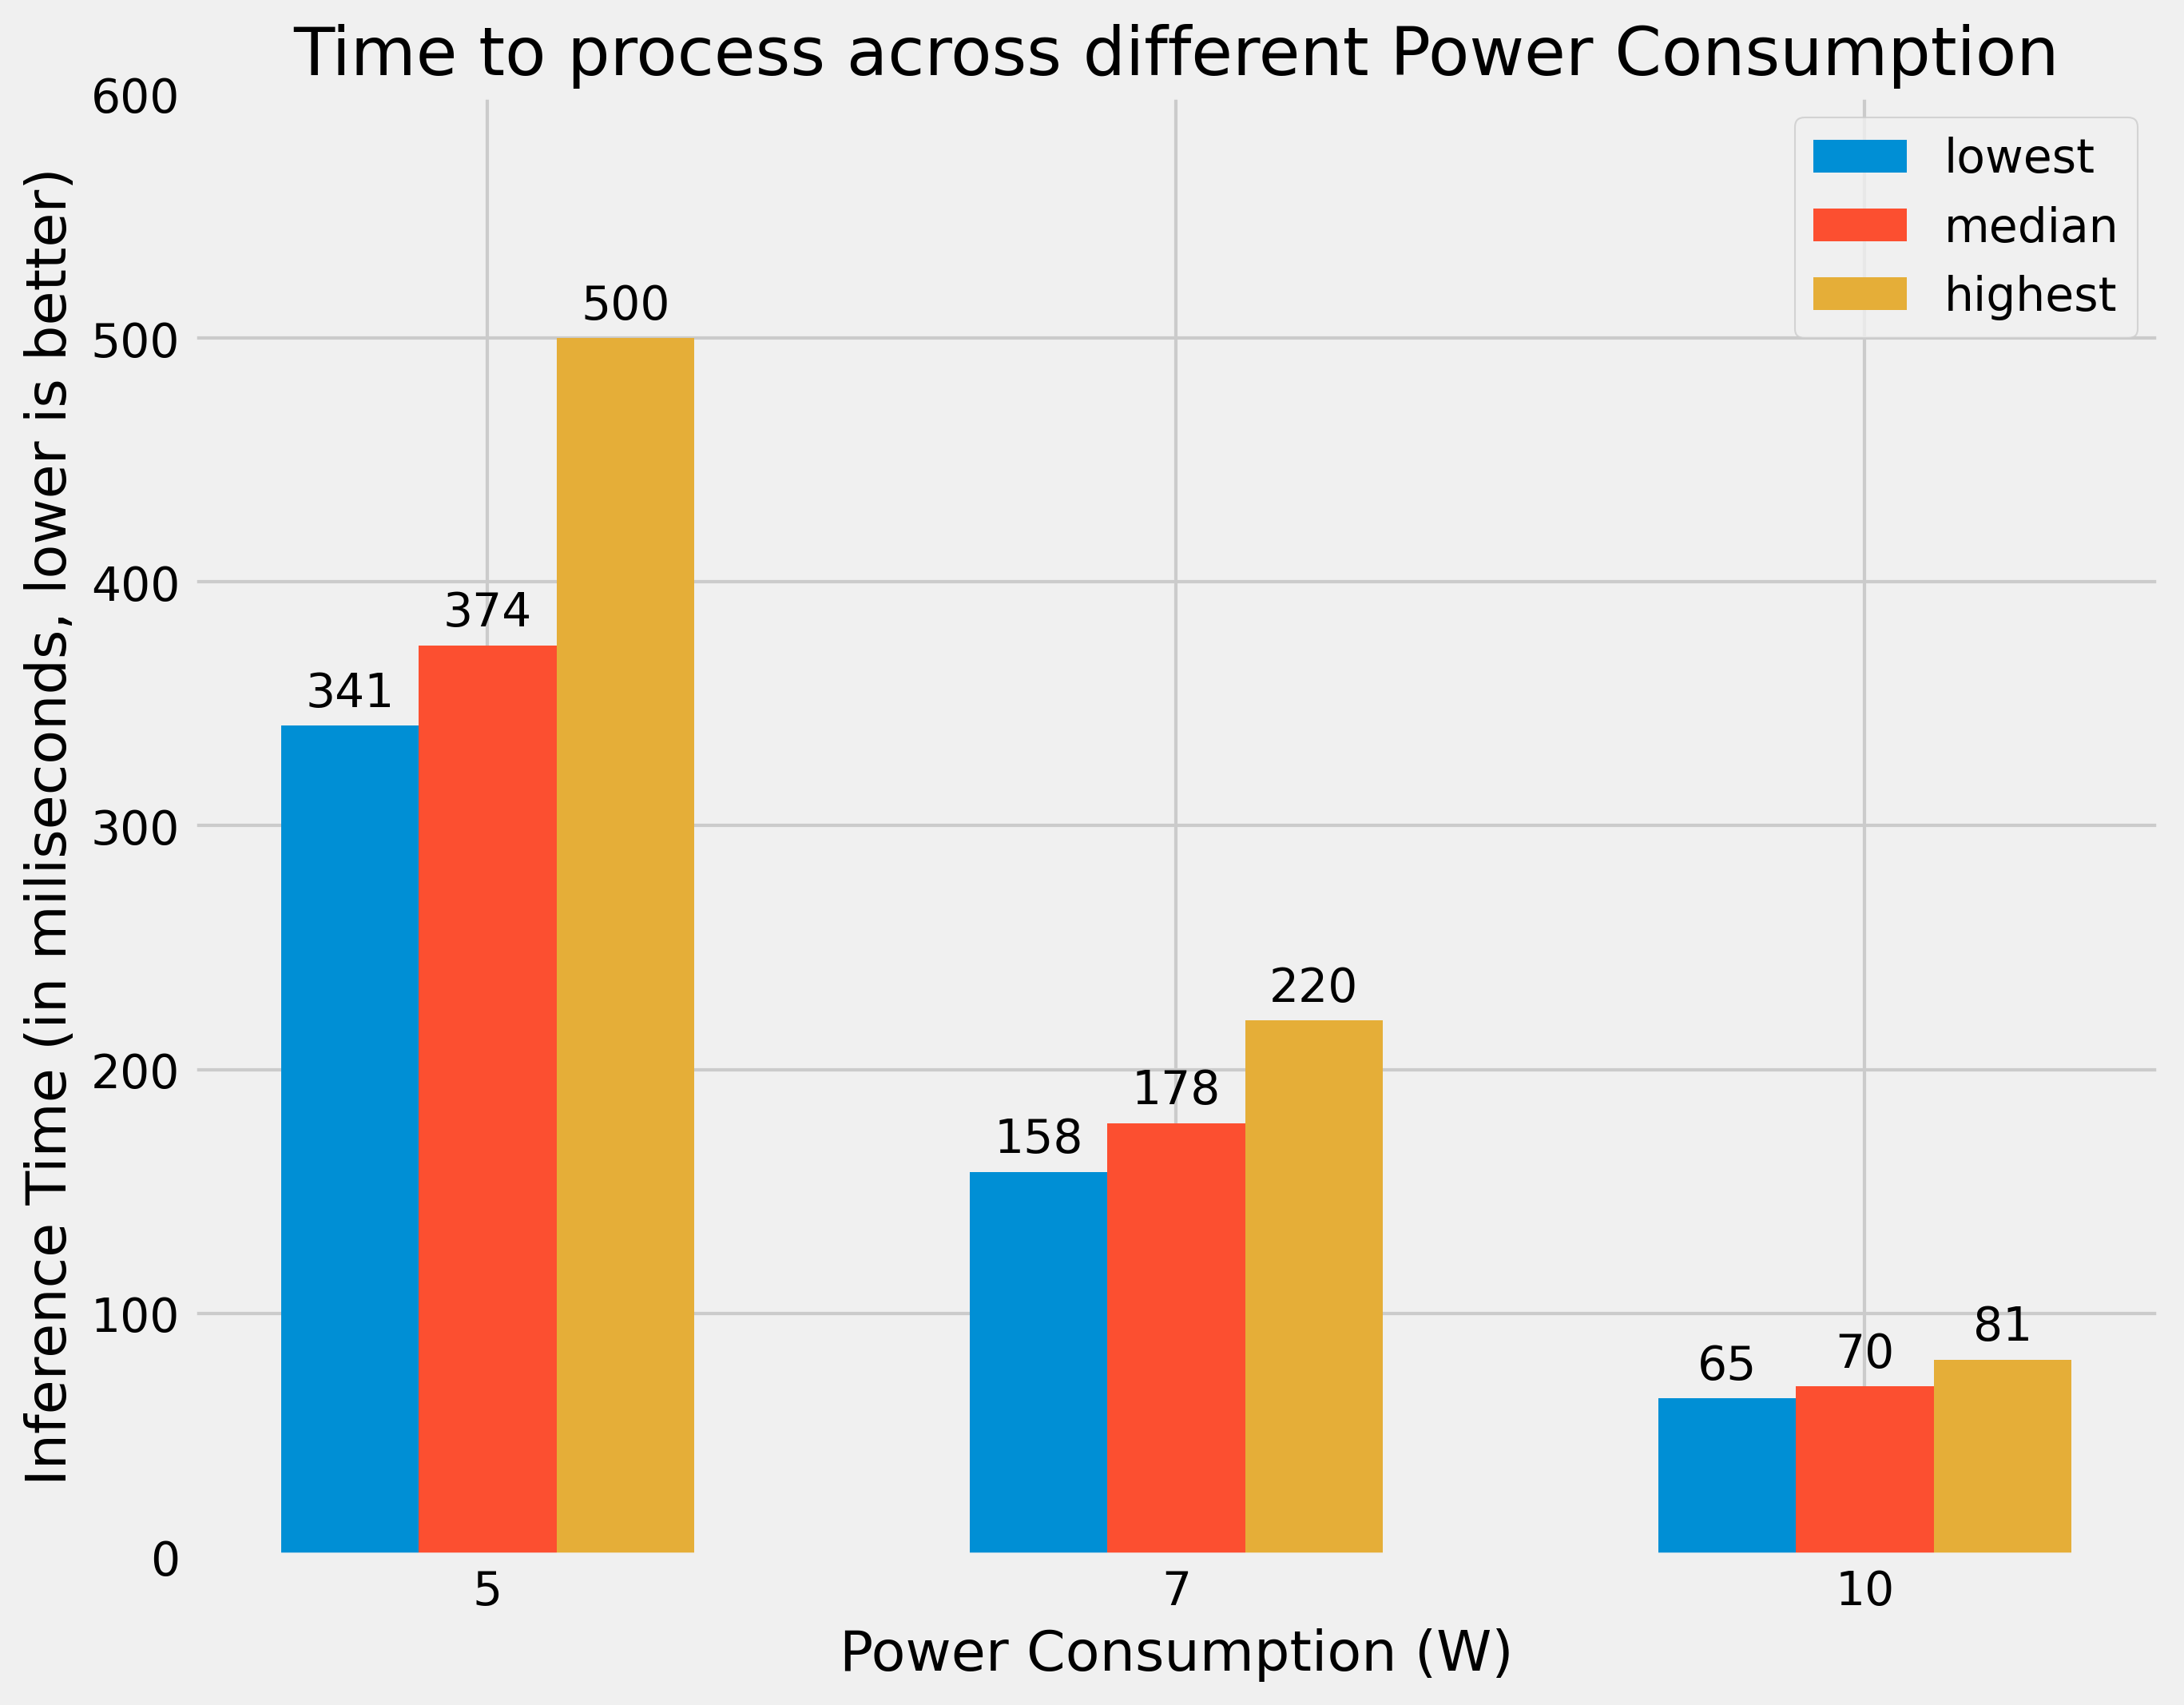
\includegraphics[width=0.5\textwidth,keepaspectratio]{inference_time_comparison.png}
\caption{Inference Time Comparison across different Power Consumption, Power Consumption error range is within 1 Watt}
\label{fig:inference_time_comparison}
\end{figure}
We also found that the Motorcycle along with its rider is the most difficult traffic object to detect. While some random red or green lights can be detected as traffic lights.
On the other hand, our system can detect Car 90\% of the time.

In terms of inference time, we gather the data by running the system in 3 different power consumption. 5 Watt, 7 Watt, and 10 Watt. We record the inference time data in miliseconds.
Many research use  FPS (Frame Per Second) as their inference process metric. We can convert inference time into FPS by using Eq \eqref{FPS}

Based on Eq \eqref{FPS} and Fig.\ref{fig:inference_time_comparison}, we can conclude that FPS and inference time are inversely proportional. As the inference time increases, the FPS decrease.
If we want to get smoother video output, we need to increase the FPS. Obviously, we need to reduce the inference time to increase the FPS.

\section{Conclusion}
Dashcam has become a popular device for drivers to record road condition. However, the dashcam video is not only used for recording the road condition, but also used for other purposes, such as insurance claims.
In this paper, we proposed a dashcam system to detect traffic objects. The object detection system is based on the YOLOv8n model. We also proposed a dataset for dashcam traffic object detection. Our dataset was created by filtering the MS COCO Dataset and adding our own annotated images. The dataset contains 78000 images with 12 traffic objects class.
By filtering dataset, we can reduce the training time and increase the model performance.
We also propose a dashcam system that can be used for testing. The system is built using Jetson Nano 4GB as the edge computer.


Based on the Real World Testing, we can conclude that our system can detect traffic object in real-world environment. Inference Time shows different results across different power consumption.
Our system power draw is  on the electrical power available in the vehicle. We managed to get the result of inference time in 3 different power consumption, 5,7, and 10 Watt.
10 Watt is the recommended power consumption for Jetson Nano 4GB. According to Nvidia, Jetson Nano 4GB can run in with MAXN mode. 
With this power consumption, our system can do the inference in under 90 miliseconds for an image size of 640x480.
While in lower power consumption, 7 Watt, our system can do the inference in around 150 - 220 miliseconds.
In 5-watt power consumption, our system can do the inference in around 340 - 500 miliseconds.
If we convert processing time into Frame Per Second, we managed to get 2 to 15 FPS.


Although using Jetson Nano was sufficient to run the system. Better performance can be achieved by using a more powerful edge computer. Such as using newer hardware from the Nvidia Jetson Series. Further optimization can be done by making use the of full potential of GPU i the Nvidia Jetson Series. Rewriting or running inference in C++ might improve the performance of the system.
Further development towards Autonomous Driving Assistance System (ADAS) can be done by adding more cameras and sensors.
\section*{Acknowledgment}
This research is supported by Telkom University, Indonesia.
We would like to personally thank M Rayhan Aryana for his help in this research.
Especially in the process of gathering the dataset and testing the system in   environment.
We also would like to thank QEngineering for open-sourcing their Jetson Nano Ubuntu 20.04 image. With their Operating System image that was preinstalled with OpenCV and Pytorch, compiled with CUDA support, we can save a lot of time in setting up the environment.



\bibliographystyle{IEEEtran}
\begin{thebibliography}{00}
\bibitem[1]{b1} A. Soin and M. Chahande, “Moving Vehicle Detection Using Deep Neural Network.” A. Soin and M. Chahande, “Moving Vehicle Detection Using Deep Neural Network.” 
\bibitem[2]{Korea Dashcam} Kim, J., Park, S., \& Lee, U. (2020). Dashcam Witness: Video Sharing Motives and Privacy Concerns Across Different Nations. IEEE Access, 8, 110425–110437. doi:10.1109/access.2020.3002079 
\bibitem[3]{Object Detection in 20 Years} https://arxiv.org/pdf/1905.05055.pdf
\bibitem[4]{b3} Krizhevsky, A., Sutskever, I., Hinton, G. E. (2012). ImageNet classification with deep convolutional neural networks. Communications of the ACM, 60(6), 84–90. https://doi.org/10.1145/3065386
\bibitem{Rich feature hierarchies} https://arxiv.org/abs/1311.2524
\bibitem{You Only Look Once} https://arxiv.org/abs/1506.02640
\bibitem{COCO Dataset} https://arxiv.org/pdf/1405.0312
\bibitem{YOLO with adaptive frame} https://link.springer.com/content/pdf/10.1007/s11042-021-11480-0.pdf
\bibitem{Road Information Collector} https://online-journals.org/index.php/i-jim/article/view/11530/6449
\bibitem{YOLOv5 ADAS} https://doi.org/10.29207/resti.v7i3.4884
\end{thebibliography}
\vspace{12pt}
\color{red}


\end{document}